\documentclass[11pt,oneside]{amsart} 
%\usepackage[utf8]{inputenc}
\usepackage[english]{babel}
\usepackage{graphicx,epsfig}
\usepackage{bbm}
\usepackage{cite}
\usepackage{amsthm}
\usepackage{esvect}
\usepackage{amsmath,amssymb,latexsym, amsfonts, amscd, amsthm, xy}
\input{xy}
\xyoption{all}

\usepackage{mathrsfs}

\usepackage{mathtools}

%options for class are \documentclass[oneside, draft]{amsart}

%\usepackage[margin=1in]{geometry}
\usepackage[margin=1.2in]{geometry}

\usepackage[dvipsnames]{xcolor}

\makeindex \setcounter{tocdepth}{2}

%\voffset = -20pt \hoffset = -60pt \textwidth = 520pt \textheighthttps://www.overleaf.com/project/5e6ade03bbf3f90001c9f74c
%=650pt \headheight = 8pt \headsep = 10pthttps://www.overleaf.com/project/5e6ade03bbf3f90001c9f74c

%\voffset = -20pt 
%\hoffset = -80pt 
%\textwidth = 520pt \textheight
%=650pt \headheight = 8pt \headsep = 10pt

%References as links
\usepackage{hyperref}
\hypersetup{pdftoolbar=true, pdftitle={GKform}, pdffitwindow=true, colorlinks=true, citecolor=blue, filecolor=black, linkcolor=purple, urlcolor=red, hypertexnames=false}
% I am having fun with this lol Z.Y.  >_<





\newtheorem{simpass}{Simplifying assumption}
\newtheorem{heegass}{Heegner assumption}

\theoremstyle{plain}
\newtheorem{iassumption}{Assumption}
\newtheorem{theorem}{Theorem}[section]
\newtheorem{conjecture}[theorem]{Conjecture}
\newtheorem{proposition}[theorem]{Proposition}
\newtheorem{corollary}[theorem]{Corollary}
\newtheorem{hypothesis}[theorem]{Hypothesis}
\newtheorem{assumption}[theorem]{Assumption}
\newtheorem*{assumption*}{Assumption}
\newtheorem{lemma}[theorem]{Lemma}
\newtheorem{question}[theorem]{Question}
\newtheorem{mainthm}{Theorem}
\newtheorem{mainrmk}[mainthm]{Remark}
\newtheorem{mainconj}[mainthm]{Conjecture}
\newtheorem{mainqz}[mainthm]{Question}

\theoremstyle{definition}
\newtheorem{definition}[theorem]{Definition}
\newtheorem{remark}[theorem]{Remark}
\newtheorem{example}[theorem]{Example}
\newtheorem*{goal*}{Goal}
\newtheorem*{problem*}{Comment}
\newtheorem{construction}[theorem]{Construction}
\newtheorem{notation}[theorem]{Notation}


\def\Gammatau{{\Gamma_{\!\tau}}}
\def\tkappa{{\tilde\kappa}}
\def\trho{{\tilde\rho}}
\def\lra{{\longrightarrow}}
\def\SL{{\bf SL}}
\def\GL{{\bf GL}}
\def\GO{{\bf GO}}
\def\GSO{{\bf GSO}}
\def\G{{\bf G}}
\def\H{{\bf H}}
%\def\O{{\bf O}}
\def\PGL{{\bf PGL}}
\def\PSL{{\bf PSL}}
\def\PP{{\mathbf P}}
\def\X{\mathbf{X}}
\def\A{\mathbb{A}}
\def\bH{\mathbb{H}}
\def\bR{\mathbb{R}}
\def\b{{\sharp}}
\def\bfeta{\boldsymbol{\eta}}

\def\bp{{x}}
\def\bpp{{y}}

\DeclareMathOperator{\can}{can}
\DeclareMathOperator{\Gr}{Gr}
\DeclareMathOperator{\OK}{\mathcal{O}_K}
\DeclareMathOperator{\NS}{NS}
\DeclareMathOperator{\Gm}{\mathbb{G}_m}
\DeclareMathOperator{\sm}{sm}
\DeclareMathOperator{\Witt}{Witt}
\DeclareMathOperator{\Tate}{Tate}
\DeclareMathOperator{\Ha}{Ha}
\DeclareMathOperator{\LL}{{\mathbb L}}
\DeclareMathOperator{\tLL}{{{\tilde {\mathbb L}}}}
\DeclareMathOperator{\tors}{tors}
\DeclareMathOperator{\cyc}{cyc}
\DeclareMathOperator{\cond}{cond}
\DeclareMathOperator{\fin}{fin}
\DeclareMathOperator{\tor}{tor}
\DeclareMathOperator{\codim}{codim}
\DeclareMathOperator{\Ext}{Ext}
\DeclareMathOperator{\mhs}{mhs}
\DeclareMathOperator{\res}{res}
\DeclareMathOperator{\comp}{comp}
\DeclareMathOperator{\ext}{Ext} 
\DeclareMathOperator{\Pic}{Pic}
\DeclareMathOperator{\Fil}{Fil} 
\DeclareMathOperator{\Rep}{{\bf Rep}}
\DeclareMathOperator{\MF}{{\bf MF}}
\DeclareMathOperator{\sym}{Sym} 
\DeclareMathOperator{\DR}{dR}
\DeclareMathOperator{\Hdg}{Hdg}\DeclareMathOperator{\GR}{gr}
\DeclareMathOperator{\dR}{dR} \DeclareMathOperator{\pr}{pr}
\DeclareMathOperator{\id}{id} \DeclareMathOperator{\Sel}{Sel}
\DeclareMathOperator{\cris}{cris}
\DeclareMathOperator{\Det}{Det}
\DeclareMathOperator{\st}{st}
\DeclareMathOperator{\Graph}{Graph}
\DeclareMathOperator{\Bl}{Bl}
\DeclareMathOperator{\disc}{Disc} \DeclareMathOperator{\cl}{cl}
\DeclareMathOperator{\Cl}{Cl}
\DeclareMathOperator{\CaCl}{CaCl}
\DeclareMathOperator{\et}{et} \DeclareMathOperator{\Norm}{Norm}
\DeclareMathOperator{\rec}{rec} \DeclareMathOperator{\Div}{Div}
\DeclareMathOperator{\Hom}{Hom}
\DeclareMathOperator{\Hombf}{{\bf Hom}}
\DeclareMathOperator{\norm}{Norm}
\DeclareMathOperator{\End}{End} \DeclareMathOperator{\CH}{CH}
\DeclareMathOperator{\AJ}{AJ} \DeclareMathOperator{\Aut}{Aut}
\DeclareMathOperator{\Stab}{Stab}
\DeclareMathOperator{\spec}{Spec} \DeclareMathOperator{\sgn}{sign}
\DeclareMathOperator{\sign}{sign} \DeclareMathOperator{\spf}{Spf} 
% \DeclareMathOperator{\ker}{ker}
\DeclareMathOperator{\coker}{coker} \DeclareMathOperator{\Tr}{Tr}
\DeclareMathOperator{\ord}{ord} \DeclareMathOperator{\univ}{univ}
\DeclareMathOperator{\Id}{Id} \DeclareMathOperator{\Int}{Int}
\DeclareMathOperator{\cusps}{cusps}
\DeclareMathOperator{\Disc}{Disc} \DeclareMathOperator{\real}{Re}
\DeclareMathOperator{\imag}{Im} \DeclareMathOperator{\frob}{Frob}
\DeclareMathOperator{\BS}{BS}
\DeclareMathOperator{\lcm}{lcm} \DeclareMathOperator{\red}{red}
\DeclareMathOperator{\tf}{\mathrm{tf}}
\DeclareMathOperator{\ddd}{d} \DeclareMathOperator{\dlog}{dlog}
\DeclareMathOperator{\art}{art} \DeclareMathOperator{\Frob}{Frob}
\DeclareMathOperator{\rank}{rank} \DeclareMathOperator{\rig}{rig}
\DeclareMathOperator{\la}{la}
\DeclareMathOperator{\ad}{ad}
\DeclareMathOperator{\tr}{t}
\DeclareMathOperator{\ur}{ur}
\DeclareMathOperator{\oor}{or}
\DeclareMathOperator{\vol}{vol}
\DeclareMathOperator{\Katz}{Katz}
\DeclareMathOperator{\Isog}{Isog}
\DeclareMathOperator{\heeg}{heeg}
\DeclareMathOperator{\Ell}{Ell}
%\DeclareMathOperator{\path}{path}
\DeclareMathOperator{\perf}{perf}
\DeclareMathOperator{\Span}{Span}
\DeclareMathOperator{\KS}{KS}
\DeclareMathOperator{\PHS}{\mathrm{PHS}}
\DeclareMathOperator{\Alg}{\bf Alg}
\DeclareMathOperator{\Rings}{\bf Rings}
\DeclareMathOperator{\an}{an}
\DeclareMathOperator{\ran}{ra}
\DeclareMathOperator{\Hodge}{Hodge}
\DeclareMathOperator{\im}{Im}
\DeclareMathOperator{\PD}{PD}
\DeclareMathOperator{\pure}{pure}
\DeclareMathOperator{\orb}{orb}
\DeclareMathOperator{\stab}{stab}
\DeclareMathOperator{\old}{old}
\DeclareMathOperator{\diiv}{div}
\DeclareMathOperator{\har}{har}
\newcommand{\VG}{\mathcal{V}(\mathcal{G})}
\newcommand{\VE}{\mathcal{E}(\mathcal{G})}
\newcommand{\Ve}{\mathcal{E}^{\oor}(\mathcal{G})}
\newcommand{\VT}{\mathcal{V}(\mathcal{T})}
\newcommand{\ET}{\mathcal{E}(\mathcal{T})}
\newcommand{\eT}{\mathcal{E}^{\oor}(\mathcal{T})}

\DeclareMathOperator{\sq}{\tilde}

 \newcommand{\dd}{\ddd\!}
\newcommand{\mat}[4]{\left( \begin{array}{cc} {#1} & {#2} \\ {#3} & {#4}
\end{array} \right)}
\newcommand{\dint}[4]{\int_{#1}^{#2}\!\!\!\int_{#3}^{#4} \!\! \dlog\alpha}
\newcommand{\dinttry}[4]{\int_{#1}^{#2}\!\!\!\int_{#3}^{#4} \!\! \dlog\alpha^{?}}
\newcommand{\mint}{\times\!\!\!\!\!\!\int}
\newcommand{\dmint}[4]{\mint_{#1}^{#2}\!\!\!\int_{#3}^{#4} \!\! \dlog\alpha}


\def\uomega{{\underline{\omega}}}
\def\spl{\Psi}
\def\fa{\mathfrak{a}}
\def\fat{{\tilde{\mathfrak{a}}}}
\def\fb{\mathfrak{b}}
\def\fc{\mathfrak{c}}
\def\ff{\mathfrak{f}}
\def\fr{\mathfrak{r}}
\def\fo{\mathfrak{o}}
\def\fp{\mathfrak{p}}
\def\fP{\mathfrak{P}}
\def\fm{\mathfrak{m}}
\def\fn{\mathfrak{n}}
\def\fD{\mathfrak{D}}
\def\fd{\mathfrak{d}}
\def\fq{\mathfrak{q}}
\def\fqb{\bar{\mathfrak{q}}}
\def\cN{\mathcal{N}}
\def\cZ{\mathcal{Z}}
\def\fN{\mathfrak{N}}
\def\d{\mathrm{d}}
\def\H{\mathbb{H}}
\def\TT{\mathbf{T}}
\def\Z{\mathbb{Z}}
\def\zq{\mathbb{Z}_q}
\def\F{\mathbb{F}}
\def\u{\mathbf{u}}
\def\E{\mathbf{E}}
\def\I{\mathbf{I}}
\def\Q{\mathbb{Q}}
\def\W{\mathbf{W}}
\def\J{\mathbf{J}}
\def\sL{\mathscr{L}}
\def\Jo{\mathbf{J}^{\vee,\circ}}
\def\V{\mathbf{V}}
\def\C{\mathbb{C}}
\def\G{\mathbb{G}}
\def\bN{\mathbf{N}}
\def\R{\mathbf{R}}
\def\P{\mathbf{P}}
\def\CC{\mathbf{C}}
\def\pp{\mathbf{P}^1}
\def\utau{\underline{\tau}}
\def\uQ{\underline{Q}}
\def\bdf{\begin{defn}}
\def\edf{\end{defn}}
\def\cM{\mathcal{M}}
\def\cL{\mathcal{L}}
\def\cH{\mathcal{H}}
\def\h{\mathcal{C}}
\def\cO{\mathcal{O}}
\def\cT{\mathcal{T}}
\def\cU{\mathcal{U}}
\def\cA{\mathcal{A}}
\def\cV{\mathcal{V}}
\def\cD{\mathcal{D}}
\def\cG{\mathcal{G}}
\def\cW{\mathcal{W}}
\def\cE{\mathcal{E}}
\def\rem{\noindent{\bf Remark.\ }}
\def\di{\displaystyle}
\def\crc{\cc\otimes_\rr\cc}
\def\gr{\mathfrak{\rho}}
\def\wu{(\gr_1,\gr_1')}
\def\hs{\hskip 2cm}
\def\sk{\vskip 0.2cm}
\def\Gal{{\rm Gal}}
\def\PGL{{\rm PGL}}
\def\corr{{\rm Corr}}
\def\gal{{\rm Gal}}
\def\ra{\rightarrow}
\def\pnew{{\rm p-new}}
\def\ux{{\underline{x}}}
\def\uy{{\underline{y}}}
\def\ab{{\rm ab}}
% \def\sha{{L\!\!L\!\!I}}
 \font\cyr=wncyr10
\def\sha{\mbox{\cyr X}}
\def\Meas{{\rm Meas}}
\def\N{\mathrm{N}}
\def\bmu{\bar{\mu}}
\def\tb{\tilde{B}}
\def\cB{{\mathcal B}}
\def\cC{{\mathcal C}}
\def\cF{{\mathcal F}}
\def\gl{\text{gl}}
\def\loc{\text{loc}}
\def\ram{\text{ram}}
\def\ab{\text{ab}}
\def\dc{d^\times}
\def\Lp{\mathcal{L}_p}
\def\di{{\bf d}}
\def\vs{\varsigma}
\def\vt{\vartheta}
\def\si{\sigma}
\def\rs{r_\sigma}
\def\vsb{\bar{\vs}}
\def\fj{\mathfrak{j}}
\def\cI{\mathcal{I}}
\def\ac{\text{ac}}
\def\d1{d^{(1)}}
\def\di{d}
\def\ve{\varepsilon}
\def\fg{\mathfrak{g}}
\def\psis{{\psi^*}}
\def\fpb{\bar{\fp}}
\def\bA{\mathbb{A}}
\def\cX{{\mathcal X}}
\def\Gm{{\mathbb{G}_m}}
\def\Gmh{{\hat{\mathbb{G}}_m}}
\def\vrt{\tilde{\varrho}}
\def\vst{\tilde{\varsigma}}
\def\vtt{\tilde{\vartheta}}
\def\bxi{{\boldsymbol{\xi}}}
\def\nablat{\tilde{\nabla}}

\def\bun{\overline{\mathbf{n}}}
\def\bln{\underline{\mathbf{n}}}
\def\d{\mathbf{d}}
\def\GG{\mathbf{G}}
\def\U{\mathbf{U}}
\def\Y{\mathbf{Y}}
\def\a{\mathbf{a}}
\def\bu{\mathbf{u}}
\def\bv{\mathbf{v}}
\def\SO{{\bf SO}}
\def\etapb{\overline{\eta'}}
\def\pdz{\frac{\partial}{\partial z}}
\def\pdzb{\frac{\partial}{\partial \bar{z}}}
\def\etapqb{\overline{\eta'_q}}
\def\RR{\mathcal{R}}
\def\MON{\mathrm{M}_0(N)}

\def\oh{\mathcal{O}}
\def\longhookrightarrow{\lhook\joinrel\longrightarrow}


%Diagrams
\usepackage{tikz}
\usetikzlibrary{positioning} 
\usepackage{tikz-cd}
\usetikzlibrary{arrows,graphs,decorations.pathmorphing,decorations.markings}


\tikzset{
commutative diagrams/.cd,
arrow style=tikz,
diagrams={>=latex}}



\setcounter{tocdepth}{1}
\begin{document} 

 \title[Geometric Quadratic Chabauty]{\small Geometric Quadratic Chabauty over Number Fields}
\author{Pavel \v{C}oupek, David Lilienfeldt, Luciena X. Xiao, Zijian Yao}
%\thanks{DL partially supported by an Alexis and Charles Pelletier Fellowship.}
\address[Pavel \v{C}oupek]{Department of Mathematics, Purdue University}
\email{pcoupek@purdue.edu}
 \address[David Lilienfeldt]{Department of Mathematics, McGill University}
\email{david.lilienfeldt@mail.mcgill.ca}
 \address[Luciena X. Xiao]{Department of Mathematics, California Institute of Technology}
\email{lucienaxiao@gmail.com}
\address[Zijian Yao]{Department of Mathematics, Harvard University}
\email{zijian.yao.math@gmail.com}
%\date{\today}
\maketitle

\begin{abstract}
We extend the method of geometric quadratic Chabauty, initiated over $\Q$ by Edixhoven and Lido, to curves of genus at least $2$ defined over arbitrary number fields. This provides a conditional bound on the number of rational points of such curves. %We give several applications of our method.
\end{abstract}


\tableofcontents
 
\vspace*{-1cm}
\section{Introduction} 

%Test: good work guys! 
 
\subsection{Chabauty--Coleman}\label{ss:CC_method}
Let $C = C_K$ be a curve of genus $g \ge 2$ defined over a number field $K$. The theorem of Faltings states that the set of rational points on $C$ is finite. Faltings's spectacular proof, however, cannot be made effective and there is no general algorithm to determine the set $C(K)$ at present. On the other hand, if the Mordell--Weil rank $r$ of the Jacobian $J$  of $C$ satisfies the inequality  
$r \le g -1$,  the pioneering work of Chabauty and Coleman  \cite{chab41, coleman}  can be used to give upper bounds for $C(K)$, and in many cases, to explicitly compute these rational points. 
Let us momentarily set $K = \Q$ and briefly explain their strategy. Upon choosing a prime $p$ of good reduction, one obtains a homomorphism 
$$\log: J (\Q_p) \lra H^0 (C_{\Q_p}, \Omega^1)^{\vee} \cong H^0 (J_{\Q_p}, \Omega^1)^{\vee} $$
induced from a linear pairing 
$J(\Q_p) \times H^0 (J_{\Q_p}, \Omega^1) \longrightarrow \Q_p$ which sends $(P, \omega)$ to the Coleman integral $\int_{0}^P \omega$. The Abel--Jacobi map $j_b: C \ra J$, after fixing a base point $b \in C(\Q)$, then leads us to the following diagram, which lies in the central spot of the method: 
\[
\begin{tikzcd}[column sep = 3em] 
C(\Q) \arrow[r] \arrow[d] & C(\Q_p)  \arrow[d] \arrow[rd, "\int"] \\
J(\Q) \arrow[r] & J (\Q_p)   \arrow[r, "\log"] & H^0 (C_{\Q_p}, \Omega^1)^{\vee}.
\end{tikzcd}
\]
The Chabauty condition $r \ge g - 1$ guarantees that the closure $Z : = \overline{J(\Q)}^p$ of $J(\Q) \subset J (\Q_p)$ with respect to the $p$-adic topology has positive codimension. In particular, there exists a nontrivial differential form $\omega$ which vanishes on $Z$. Roughly, $\omega$ is locally given by a $p$-adic power series and has only finitely many zeroes on each residue disk of $C(\Q_p)$. Therefore, the intersection $J(\Q) \cap C(\Q_p)$, thus $C(\Q)$, is finite. Moreover, the computation of $C(\Q)$ amounts to computing these power series to sufficient $p$-adic precision on each residue disk.  

\subsection{Quadratic Chabauty}
The fascinating program initiated by Kim (see \cite{Kim05, Kim09}) aims to relax the Chabauty condition by considering non-abelian variants of the objects in \S \ref{ss:CC_method}. To this end, we first reinterpret the diagram above using the Bloch--Kato selmer groups $H^1_f(\Q, V)$ (resp. $H^1_{f} ( {\Q_p}, V)$) in place of $J(\Q)$ (resp. $J(\Q_p)$) via the Kummer maps, where $V := H^1_{\text{\'et}}(C_{\overline \Q}, \Q_p)^\vee$ is the $p$-adic \'etale cohomology of $C$. The logarithm map above is essentially the inverse of the Bloch--Kato exponential 
$$ H^0 (C_{\Q_p}, \Omega^1)^\vee \cong \textup{D}_{\textup{dR}} (V)/\textup{D}^+_{\textup{dR}} (V) \xrightarrow{\:\: \text{ exp } \:\:} H^1_f (\Q_p, V).$$
Next, we replace $V$ by certain pro-unipotent quotients $U_n$ of the \'etale fundamental group $\pi_1^{\text{\'et}} (C_{\overline \Q})_{\Q_p}$, one for each $n \ge 1$, which again carries a continuous action by $\textup{Gal}_{\Q}$. Kim defines a certain Selmer subgroup $\textup{Sel}(U_n) \subset H^1_f (\Q, U_n)$, and upgrades the previous diagram to 
\[
\begin{tikzcd}[column sep = 2em] 
C(\Q) \arrow[r] \arrow[d, "j_n"] & C(\Q_p)  \arrow[d, "j_{n, p}"] \arrow[rd, "\int"] \\
\textup{Sel}(U_n) \arrow[r, "\textup{loc}_p"] & H^1_{f} (\Q_p, U_n)  \arrow[r, "\log_n"] & \pi_1^{\textup{dR}} (C_{\Q_p})_{n}/ \textup{Fil}^0.
\end{tikzcd}
\]
Here the vertical maps $j_n$ and $j_{n, p}$ are Kim's unipotent Kummer maps. %In fact, all objects in this diagram have natural structures of algebraic varieties and the bottom arrow comes from maps of such varieties. 
The intersection $J(\Q) \cap C(\Q_p)$ in the Chabauty--Coleman method is now replaced by the set
$$ C(\Q_p)_n : = j_{n, p}^{-1} \big(\textup{loc}_p (\textup{Sel}(U_n))\big)  $$
that contains $C(\Q)$. For sufficiently large $n$, Kim conjectures that $C(\Q_p)_n$ is finite, and even coincides with $C(\Q)$. The first instances of Kim's program have been carried out quite successively by Balakrishnan and her collaborators. In particular, for the quadratic case where $n = 2$, if the Mordell--Weil rank $r$ satisfies $r \le g + \rho - 2$ where $\rho$ is the rank of the N\'eron--Severi group of $J$, then $C(\Q_p)_2$ is finite and can often be explicitly determined (see \cite{BD18a, BD19} and references therein).  This method has been successfully applied to determine rational points on the ``cursed curve'' in \cite{balakrishnan2019}, which finishes the classification of non-CM elliptic curves over $\Q$ of split Cartan type. 

Recently, a different, less cohomological but probably more direct approach to quadratic Chabauty has been found by Edixhoven--Lido. Their idea is to consider a certain $\Gm$-torsor $T$ over the Jacobian instead of the Selmer variety $\textup{Sel}(U_2)$. Their method is expected to work under the same quadratic Chabauty condition $r \le g+\rho - 2$, but has the advantage of avoiding the consideration of iterated Coleman integrals and the analysis of certain complicated $p$-adic heights. In fact, this method is rather geometric and elementary, and even eliminates the language of (non-abelian) $p$-adic Hodge theory used by Kim. 

\subsection{Quadratic Chabauty over number fields} \label{ss:other_work_K}
On a different direction, a natural question is how to generalize the Chabauty--Coleman method and its non-abelian variants to more general number fields $K$. 

To put this article into context, we briefly recall the first steps towards such generalizations studied by \cite{siksek, BBBM19, Dogra19}. In order to  apply the idea of Chabauty--Coleman, Siksek \cite{siksek} considers the Weil restriction $\textup{Res}_{K/\Q} J$ and studies Coleman integration in this context. The work of \cite{BBBM19} builds on this idea and studies rational points on hyperelliptic curves satisfying a more relaxed Chabauty condition compared to \cite{siksek} (also see \S \ref{s:chabcondition}). The work of Dogra \cite{Dogra19}, on the other hand, is directly related to the approach of Kim, relying on a certain arithmetic form of quadratic Chabauty condition (see Remark \ref{remark:chabcondition}). We refer the interested reader to  \cite{Dogra19} for more details on his results. 

\subsection{Main result}
In this article and subsequent works, we generalize the geometric approach initiated by Edixhoven--Lido to arbitrary number fields. Our main theoretical result in this article is roughly the following 

\begin{mainthm} \label{thm:intro_main}
Let $K$ be a number field of degree $d = r_1 +2 r_2$, where $2r_2$ is the number of complex embeddings of $K$.  Let $C_K$ be a smooth proper geometrically connected curve of genus $g \ge 2$ with Mordell--Weil rank $r$ over $K$, satisfying
 \begin{equation} \label{eq:geom_cc}
  r \le d(g-1) + (\rho - 1) (r_2 + 1),
  \end{equation}
 where $\rho$ is the rank of the N\'eron--Severi group of the Jacobian $J_K$. Let $\delta : = r_1 + r_2 - 1$ and 
 $$ A := \Z_p \langle z_1, ..., z_{\delta (\rho - 1)+ r} \rangle $$
 be the $p$-adically completed polynomial algebra over $\Z_p$. There exists an explicitly computable ideal $I$ of $A$, such that if $\overline A:= A/I \otimes \F_p$ is a finite dimensional $\F_p$ vector space, then the set of rational points $C_K(K)$ is finite and bounded above by $\dim_{\F_p} \overline A$. 
 \end{mainthm}
In this case we expect $C_K (K)$ to be explicitly computable. 

\begin{mainrmk} \label{remark:main_intro}
The precise form of the main theorem (Theorem \ref{thm:main_rough_form}) is slightly more involved than what is stated above. For example, in order for our method to work, we need to ``cover'' $C_K$ by certain open subschemes $U_i$ and work with one $U_i$ at a time. In particular, we shall construct an ideal $I_i \subset A$ to bound the rational points on $U_i$ for each $i$.  
\end{mainrmk}

\begin{mainrmk}
The condition (\ref{eq:geom_cc}), which we refer to as the geometric quadratic Chabauty condition (Definition \ref{definition:chabcondition}), is the ``best bound'' for explicit quadratic Chabauty methods over number fields in literature. See \S \ref{s:chabcondition} for comparisons with other Chabauty bounds that arise in the aforementioned works in \S \ref{ss:other_work_K}. 
\end{mainrmk}
 
 
\subsection{Overview of the approach}
Now we briefly explain the idea of geometric quadratic Chabauty, which we extend from \cite{EL19}.  
As is the case of the methods of Chabauty--Coleman and Chabauty--Kim, the nature of this approach is inherently $p$-adic. Let $p$ be a prime of good reduction for the curve $C_K$. The strategy is to replace the Jacobian in Chabauty's original approach by something higher dimensional in order to play the Chabauty game. Slightly more precisely, we will construct a certain $\G_m^{\rho-1}$-torsor $T_K$ over $J_K$, where $\rho$ is as defined in Theorem \ref{thm:intro_main}, which will replace $J_K$. This, however, introduces ``too many rational points'' as the fiber of $T_K$ over $J_K$ is $\Gm^{\rho - 1}$ and $\Gm(K) = K^\times$ is not finitely generated, thus it is more natural to consider an integral model $\CC$ of $C_K$ over the ring of integers $\oh_K$. 

In other words, we shall construct a certain $\Gm^{\rho-1}$-torsor $\TT$ over the $\J$, the latter being the N\'eron model of $J_K$. % over $\oh_K$. This way, over each $\oh_K$-point of $\J$, we have introduced $\Gm^{\rho - 1} (\oh_K)= (\oh_K^\times)^{\rho- 1}$ worth of $\oh_K$-points. 
%For notational simplification, let us assume that $K$ is a quadratic extension of $\Q$ and $p$ an inert prime. 
%The idea is then to carefully pick a certain finite cover of (the smooth locus of) $\CC$ by $\U_i$, each of which admits a lift to the torsor $\TT$  %\[ \begin{tikzcd}  & \TT \arrow[d] \\ \U_i \arrow[ru, hook, "\tilde j_b^i"]  \arrow[r, hook, "j_b"] & \J \end{tikzcd} \]
The idea is then to carefully lift the Abel--Jacobi map $j_b: \CC \ra \J$ to the torsor $\TT$
\[
\begin{tikzcd}[row sep = 1em]  & \TT \arrow[d] \\ \CC \arrow[ru, "\tilde j_b"]  \arrow[r, hook, "j_b"] & \J \end{tikzcd} 
\]
% We then work with one such $\U_i$ at a time, which we fix in the introduction and call it $\U$.  
We then consider $\CC (\oh_K) \subset \CC (\oh_{K, p})$ as a subset of the $p$-adic points, where $\oh_{K, p} := \oh_K \otimes_{\Z} \Z_p$, and arrive at the following ``quadratic Chabauty diagram" over $\oh_K$
\begin{equation} \label{diagram:intro}
 \begin{tikzcd}  \CC(\oh_{K})  \arrow[d,  "\tilde j_b"]  \arrow[rr] &&  \CC(\oh_{K, p}) \arrow[d] \\   \TT(\oh_K)  \arrow[r] & \Y \arrow[r]   & \TT(\oh_{K, p}) \end{tikzcd}. 
 \end{equation}
Here $\Y := \overline{\TT(\oh_K)}^p$ is the closure of $\TT(\oh_K)$ in $\TT(\oh_{K, p})$ for the $p$-adic topology. 
As in \S \ref{ss:CC_method}, the rational points $C_K (K) = \CC(\oh_K)$ is contained in  $ \CC(\oh_{K, p})  \cap \Y,$ which is often finite and computable. 

The key of this approach is thus to analyze the $p$-adic closure $\Y$ of the $\oh_K$-points of the torsor $\TT$. If $K = \Q$, then this can be done via parametrizing the $p$-adic closure of $\J(\Z) = J (\Q)$, as $\Gm (\Z) = \pm 1$. This is a major simplification and essentially why \cite{EL19} decides to work over $\Q$. In fact, it was suggested to us by the authors of \cite{EL19} that an approach similar to that of \cite{siksek} might reduce the case of general number fields $K$ back to the case of $\Q$. In this article, however, we decide to take a slightly more direct approach, as one of our main observations is that one can in fact fully utilize the $\Gm$-action on the fibers of the torsor $\TT \rightarrow \J$ to parametrize $\Y$, which is sufficient for our purpose. Roughly, we pick a ``$\Z$-coordinate'' map $\Z^{r} \ra \TT(\oh_K)$ essentially by choosing basis for the Mordell--Weil group $J(K)$. We then use the $\Gm$-action to propagate these coordinates to get a  ``$\Z$-coordinate'' map $\Z^{\delta(\rho - 1) + r} \ra \TT(\oh_K)$, where $\delta$ is as defined in Theorem \ref{thm:intro_main}. Finally, $p$-adically interpolating these coordinates allow us to parametrize $\Y$ via a surjective map $$\kappa: \Z_p^{\delta (\rho - 1)+r} \longrightarrow \Y, $$ 
which turns out to be given by convergent $p$-adic power series. In fact, the ideal $I$ from Theorem \ref{thm:intro_main} is built such that the cardinality of  $\spec \overline{A}$ measures the size of $\kappa^{-1} (\Y \cap \CC(\oh_{K, p}))$. In particular, in order for our method to be able to explicitly determine the rational points on $C_K$, we need to choose a prime $p$ such that  
\begin{itemize} 
\item $\Y \cap \CC (\oh_{K, p})$ is finite
\item $\kappa$ is ``finite-to-one'' on $\kappa^{-1} (\Y \cap \oh_{K, p})$. 
\end{itemize}
We conjecture that the first outcome is always achieved, and hope that there exists a good $p$ such that the second condition is also satisfied. 

\begin{mainconj}
Let $p$ be a prime of good reduction for $C_K$, then the intersection $\Y \cap \CC(\oh_{K, p})$ as in the commutative diagram (\ref{diagram:intro}) is finite. 
\end{mainconj} 

\begin{mainqz} \label{question:intro}
For a given curve $C_K$, does there always exist a prime $p$ such that the ring $\overline A$ as in Theorem \ref{thm:intro_main} is finite dimensional over $\F_p$.
\end{mainqz}

%(see also Theorem \ref{thm:main_rough_form} for the meaning of the subscript $i$) is finite dimensional over $\F_p$ for each $i$. 
%We then further break down the computation in residue disks. In other words, consider the map  $$\U(\oh_{K, p}) \ra  \U(\F_q)$$ where $\F_q = \oh_K/p$ is the residue field (and in this case $q = p^2$). We consider one residue disk at a time. Namely, for each $u \in \U (\F_q)$, we denote $\U(\oh_{K, p})_{u}$ the residue disk above $u$ and $\U(\oh_{K})_u$ its intersection with $\U(\oh_K)$.  Let $b = \tilde j_b (u) \in \TT (\oh_K)$, then we arrive at the following diagram  \[ \begin{tikzcd}  \U(\oh_{K})_t  \arrow[d, hook]  \arrow[r, hook] & \TT(\oh_K)_b \arrow[d, hook] \\ \U(\oh_{K, p})_t   \arrow[r, hook, "\tilde j_b"] & \TT(\oh_{K, p})_t \end{tikzcd} \]  The upshot is that the rational points $\U(\oh_K)_t$  in the residue disk above $t$ is contained in  $$ \U(\oh_{K, p})_t  \cap \overline{\TT(\oh_K)_b}^{p} \longhookrightarrow \TT(\oh_{K, p})_t $$  where $ \overline{\TT(\oh_K)_b}^{(p)}$ denotes the closure of the rational points in $p$-adic polydisk $\TT(\oh_{K, p})_t$, and at the same time the intersection is often finite and computable. 

\begin{mainrmk} 
There are, of course, further caveats hidden from the over-simplified overview above. For example, as hinted in Remark \ref{remark:main_intro}, in order to obtain the lifting $\widetilde j_b: \CC \ra \TT$, we need to restrict to certain open subscheme $\U_i$ of the smooth locus $\CC^{\sm}$ inside $\CC$. Moreover, when constructing $\kappa$, we will work on one residue disk inside each $\U_i(\oh_{K, p})$ at a time. The details of these complications are spread in the article, for example see \S \ref{trivialization} and \S \ref{s:construct}. In particular, a precise form of Question \ref{question:intro} is formulated in \S \ref{sec:bound}. 
\end{mainrmk}

\subsection{Outline}

In the end of this introduction let us briefly outline the content of each section. In \S \ref{s:torsor} we recall some basic background on the Poincar\'e torsor, from which we build the torsor $T_K$ over $J_K$ mentioned in the overview above. We then spread out the entire picture from $\spec K$ to $\spec \oh_K$ to obtain a precise version of diagram (\ref{diagram:intro}). Then, in \S \ref{s:method}, we give more details of the strategy of geometric quadratic Chabauty, before stating the main technical results of this article. We also explain how the geometric quadratic Chabauty condition arises and discuss how it specializes to conditions that appear in the ``classical" quadratic Chabauty method that is part of Kim's program. In \S \ref{s:closure}, which is the technical core of this article, we discuss how to parametrize the $p$-adic closure $\Y$ of the ``rational points'' $\TT(\oh_K)$ via a certain $p$-adic interpolation. Finally, we complete the proof of the main theoretical results in \S \ref{sec:bound}.  



\subsection*{Acknowledgements}

This project was initiated during the Arizona Winter School in March, 2020 and was proposed to us by Bas Edixhoven. We wish to thank the organizers of the conference for making this collaboration possible. We are grateful to Bas Edixhoven and Guido Lido for offering their insights and answering many of our questions regarding their paper. We thank Jan Vonk for many helpful discussions during the project.   



\subsection*{Notation} \label{ss:notation}

For the convenience of the reader we provide a list of notations used in the paper.

\begin{itemize}
\item $K/\Q$ is a number field of degree $d=r_1+2r_2$, where $r_1$ and $r_2$ are respectively the number of real embeddings and pairs of complex embeddings of $K$. 
\item $\oh_K$ denotes the ring of integers of $K$. 
\item $\delta=r_1+r_2-1$ is the rank of the unit group $\oh_K^\times$. 
\item $h=\cl(\oh_K)$ is the class number of $\oh_K$. 
\item $C_K$ is a smooth proper geometrically connected curve over $K$ of genus $g\geq 2$. 
\item $J_K=\Pic^0_{C_K/K}$ is the Jacobian of $C_K$; it is an abelian variety of dimension $g$ over $K$.
\item $J^{\vee}_{K}=\Pic^0_{J_K/K}$ is the dual abelian variety of $J_K$.
\item $P^\times_K\lra J_K\times J_K^\vee$ is the Poincar\'e torsor; it is a biextension of $J_K$ and $J_K^\vee$ by $\G_m$.
\item $\CC$ is a regular proper model of $C_K$ over $\oh_K$ that we fix in this article.
\item $\J$ is the N\'eron model of $J_K$ over $\oh_K$.
\item $\J^\vee$ is the N\'eron model of $J_K^\vee$ over $\oh_K$.
\item $\Jo$ is the fiber-wise connected component of $0$ of $\J^\vee$.
\item $\mathbf{P}^\times\lra \J\times \Jo$ is the unique biextension of $\J$ and $\Jo$ by $\G_m$ whose base change to $K$ is the Poincar\'e torsor.
\item $j_b : C_K\lra J_K$ is the Abel-Jacobi map associated to a choice of point $b\in C_K(K)$.
\item $r=\rank_{\Z} J_K(K)$ is the Mordell--Weil rank over $K$.
\item $\rho=\rank_{\Z} \NS_{J_K/K}(K)$ is the rank of the N\'eron--Severi group of $J_K$ over $K$.
\end{itemize}
 
 
 






\section{The Poincar\'e torsor} \label{s:torsor}

In this section we recall some background on algebraic geometry necessary for the method of geometric quadratic Chabauty. In particular, we briefly review the key geometric object studied in this paper, namely the Poincar\'e torsor. 


\subsection{The Poincar\'e torsor}\label{S:PicTors}

%\begin{itemize}
  %  \item { \color{violet} (Zijian) Nice choice of color David (bittersweet lol). In fact any $\mathscr L^\times$ is representable -- just cover $X$ by Zariski opens $U$ where $\mathscr L$ is trivialized. Now the open subfunctor in question is isomorphic to $\textup{Isom}_U (\oh_U, \oh_U) \cong $ the trivial $ \G_m$-torsor over $U$. More generally we always know that such Isom/Hom functors are representable by algebraic spaces, but in this case I think Zariski descent is easy since line bundles have a very easy Zariski-local description. }
   % \item {\color{Bittersweet} \color{NavyBlue} (Pavel) OK, deleting my comments since they are no longer relevant. Just note that there is still the description of functor of points, ($L^{\times}(S)$ for $S\stackrel{\varphi}{\rightarrow}X$...), only in the text now. \color{Bittersweet} Yes I left this description that you wrote originally. Let's keep it there for now.}
%\end{itemize}
\color{black}

First we recall that, given a line bundle $\mathscr{L}$ on an arbitrary scheme $X$, its associated $\Gm$-torsor is $\mathscr{L}^\times = \textbf{Isom}_X (\oh_X, \mathscr L)$, which is equipped with a natural free and transitive  action of $\Gm$. Concretely, $\mathscr{L}^\times$ is (locally) obtained by deleting the zero section of $\mathscr L$. %The association $\mathscr L  \mapsto \mathscr L^\times$ induces a bijection between (the isomorphism classes of) line bundles and $\Gm$-torsors. 
Note that $\mathscr L^\times$ is Zariski locally trivial, in particular it is represented by a scheme over $X$, which we again denote by $\mathscr L^\times$ by slightly abusing notations. 

The most relevant example for this paper is the Poincar\'e torsor for the Jacobian of a curve, which we now discuss. As in the introduction, we let $C_K$ be a smooth proper geometrically connected curve of genus $g\geq 2$ defined over $K$ and $J_K$ be its Jacobian. The dual abelian variety of $J_K$ is  $J_K^\vee$ and comes equipped with a canonical principal polarization $\lambda : J_K\overset{\sim}{\lra} J_K^\vee$ by translating the theta divisor. 
Let $P_K$ denote the Poicar\'e bundle on $J_K\times J_K^\vee$, which carries a canonical birigidification with respect to the identity sections of $J_K$ and $J_K^\vee$. More precisely, $P_K$ is canonically trivialized over $\{0 \}\times J_K^\vee$ and $J_K\times \{ 0 \}$ and these trivializations are compatible on $\{0 \}\times\{0 \}$. The Poincar\'e torsor $P_K^\times$ is the $\G_m$-torsor on $J_K\times J_K^\vee$ associated to $P_K$. As above, we again denote by $P_K^\times$ the scheme represented by the Poincar\'e torsor and  denote by $j_K : P_K^\times \lra J_K\times J_K^\vee$ the structural morphism.
%Recall from \S \ref{S:PicTors} that it is the scheme over $J_K\times J_K^\vee$ which represents the functor $\mathbf{Isom}_{J_K\times J_K^\vee}(\oh_{J_K\times J_K^\vee}, P_K)$. 
%\begin{equation}\label{def:PoinTors}
%    P_K^\times := \mathbf{Isom}_{J_K\times J_K^\vee}(\oh_{J_K\times J_K^\vee}, P_K).
%\end{equation}
%For every $(J_K\times J_K^\vee)$-scheme $\phi : S\lra J_K\times J_K^\vee$, $P_K^\times(S)$ is the set of isomorphisms of $\oh_S$-modules from $\oh_S$ to $\phi^* P_K$. It is equipped with a free and transitive action of $\G_m(S)=\oh_S(S)^\times$. The functor $P_K^\times$ is represented by a scheme over $J_K\times J_K^\vee$.

%%% The original subsection is commented below.
%%%
%%%
%%%
%  Let $X$ denote a scheme. Given a line bundle $L \rightarrow X$, we denote by $\mathscr{L}$ the corresponding sheaf on $X$. 
% One can naturally associate to $L$ a $\G_m$-torsor $L^{\times}$ on $X$ (which will locally trivialize over a Zariski open cover of $X$) defined as the open subscheme of $L$ obtained by deleting the image of the zero section. In terms of points, for a scheme    $S\stackrel{\varphi}{\rightarrow} X$ over $X$, $L^{\times}(S)$ is given as the set of isomorphisms of $\oh_S$-modules $\oh_S \rightarrow \varphi^{*} \mathscr{L}$ with the natural free and transitive action of $\G_m(S)=\oh_S(S)^{\times}$. 
%\begin{equation}
 %   \mathscr{L}^\times := \mathbf{Isom}_{X}(\oh_{X}, \mathscr{L})
%\end{equation}
%which is representable by a scheme $L^\times$ over $X$ by \cite[Theorem 4.3]{milne} as the group scheme $\G_m$ over $X$ is affine. Concretely, the $\G_m$-torsor $L^{\times}$ on $X$ can be described
%(which will locally trivialize over a Zariski open cover of $X$) 

%As $\G_m$-torsors on $X$ are classified by the \v{C}ech cohomology group $\check{H}^1(X, \G_m)$, the operation $L \mapsto L^{\times}$ describes a morphism $\Pic(X)\rightarrow \check{H}^1(X, \G_m)$ which is an isomorphism, inverse to the canonical isomorphism $\check{H}^1(X, \G_m)\rightarrow H^1(X, \G_m) \simeq \Pic(X)$; in particular, every $\G_m$-torsor on $X$ arises this way, and $\Pic(X)$ classifies isomorphism classes of $\G_m$-torsors on $X$. 



\subsection{The Poincar\'e torsor as a $\Gm$-biextension}\label{S:PoincareTorsor}

  %First note that the Poincar\'e  torsor $P_K^\times$ inherits from $P_K$ a canonical structure of a birigidified $\G_m$-torsor over $J_K\times J_K^\vee$, with respect to the identity sections of $J_K$ and $J_K^\vee$. 

In this subsection we explain the biextension structure of the Poincar\'e torsor that plays a central role in our paper. The assertion is that $P_K^\times$ admits a unique structure as a $\G_m$-biextension of the couple $(J_K, J_K^\vee)$, which is compatible with its canonical birigidified $\Gm$-torsor structure inherited from $P_K$  
(\cite[VII.Definition 2.1, Exemple 2.9.5]{SGA7}). Instead of repeating the definition from SGA 7, let us briefly explain what this means.  % without repeating the definition from SGA 7. 

%This means (see \cite[Definition 2.1]{SGA7_1(VII)}) that the $\G_m$-torsor $j_K : P_K^\times \lra J_K \times J_K^\vee$ has the following extra structures:

  \subsubsection*{$\bullet$ Partial composition $+_1$}  First, we may view $P_K^\times$ as a scheme over $J_K^\vee$ via the structure morphism $\pr_2\circ j_K$. As such, $P_K^\times$ becomes a commutative $J_K^\vee$-group scheme which is an extension of $J_{K, J_K^\vee} := J_K \times J_K^\vee$ by $\G_{m, J_K^\vee} = \Gm \times J_K^\vee$. In other words, $P_K^\times$ fits into the following short exact sequence of  $J_K^\vee$-group schemes
    \begin{equation}\label{ext1}
        1 \lra \G_{m, J_K^\vee} \lra P_K^\times \lra J_{K, J_K^\vee} \lra 0.
    \end{equation}
To wit, let $S$ be a $K$-scheme, $y \in J_K^\vee(S)$ be an $S$-point of $J^\vee_K$, and $x_1, x_2 \in J_K(S)$ be two $S$-points of $J_K$. Let $z_1, z_2 \in P_K^\vee (S)$ be two $S$-points lying above $(x_1, y)$ and $(x_2, y)$ respectively via the structure map $j_K$. This group structure can be described as follows. % (see also \cite[Section 2]{EL19}). 
The data of the point $z_1$ (resp. $z_2$) is equivalent to a nowhere vanishing section $\alpha_1 \in (x_1, y)^* P_K (S)$ (resp. $\alpha_2$) of the pullback of the Poincar\'e bundle. Now, as part of the requirement of being a $\G_m$-biextension, we have an isomorphism of line bundles over $\oh_S$
    \begin{equation}\label{eq:thm_square}
(x_1, y)^* P_K \otimes (x_2, y)^* P_K \cong (x_1+x_2, y)^* P_K,
\end{equation} (supplied by the theorem of square). 
Under this (canonical) isomorphism the tensor product  $\alpha_1 \otimes \alpha_2$ corresponds to a nowhere zero section $\alpha_3$ of $(x_1+x_2, y)^* P_K$, thus producing a point $z_3 \in P_K^\times(S)$ that lies above the point  $(x_1+ x_2, y)$ of $J_K \times J_K^\vee$. The commutativity of $P_K^\times$ as a $J_K^\vee$-group is clear, as well as the exact sequence displayed above. 
    We denote by $+_1$ the resulting \textit{partial composition law} on $P_K^\times$, which provides the group structure of $P_K^\times$ over $J_K^\vee$ (but not over $K$), in other words, it is defined on couples of points $z_1, z_2\in P_K^\times(S)$ such that $$ \pr_2(j_K(z_1))=\pr_2(j_K(z_2)).$$
   Let us also denote the group structure on the $J_K^\vee$-group scheme $J_{K, J_K^\vee}$ by $+_1$ (again slightly abusing notations), then the partial composition law $+_1$ on $P_K^\times$ satisfies
\[
 z_1 +_1 z_2 \in P_K^\times (S) \:\:  \longmapsto \: (x_1, y) +_1 (x_2, y) = (x_1+x_2, y) \in J_{K, J_K^\vee} (S). 
\]
    
  \subsubsection*{$\bullet$ Partial composition $+_2$} 
     On the other hand, we may view $P_K^\times$ as a  $J_K$-scheme via the structure morphism $\pr_1\circ j_K$. As above, this makes  $P_K^\times$ an extension of $J^\vee_{K, J_K}$ by $\G_{m, J_K}$, %(here $J^\vee_{K, J_K}$ denotes $J_K\times J_K^\vee$ viewed as a $J_K$-group scheme by pulling back the group scheme structure of $J_K^\vee\lra \spec K$ via $J_K\lra \spec K$). 
    which fits into a short exact sequence of commutative $J_K$-group schemes
    \begin{equation}\label{ext2}
        1 \lra \G_{m, J_K} \lra P_K^\times \lra J^\vee_{K, J_K} \lra 0.
    \end{equation} 
   We denote by $+_2$ the resulting partial composition law on $P_K^\times$, this time defined on couples of points $z_1, z_2 \in P_K^\times(S)$ that satisfy 
    \[ \pr_1(j_K(z_1))=\pr_1(j_K(z_2)). \]
    
   \subsubsection*{$\bullet$ Compatibility} 
    The commutative group scheme extensions (\ref{ext1}) and (\ref{ext2}) are compatible in the following sense. Let $S$ be any $K$-scheme. Let $z_\alpha, z_\beta, z_\gamma, z_\delta \in P_K^\times (S)$ be arbitrary   $S$-points such that 
    $$j_K(z_\alpha) = (x_1, y_1), \quad j_K(z_\beta) = (x_1, y_2), \quad j_K(z_\gamma) = (x_2, y_1), \quad j_K(z_\delta) = (x_2, y_2)$$
     for some $S$-points $x_1, x_2\in J_K(S)$ and $y_1, y_2\in J_K^\vee(S)$. Then
    \begin{equation}
        (z_\alpha +_2 z_\beta)+_1 (z_\gamma +_2 z_\delta)=(z_\alpha+_1 z_\gamma)+_2 (z_\beta +_1 z_\delta)
    \end{equation}
   % for all $x\in (p, q)^* P_{K}^\times(S), y\in (p, q')^* P_{K}^\times(S), z\in (p', q)^* P_{K}^\times(S)$ and $t\in (p', q')^* P_{K}^\times(S)$. (Here, $(p, q)^* P_K^\times$ is the $\G_{m, S}$-torsor over $S$ obtained from $P_K^\times$ by pull-back via $(p, q) : S\lra J_K \times J_K^\vee$). 
We summarize this compatibility in the following picture for the convenience of the reader. 

\begin{center}
\tikzset{every picture/.style={line width=0.7pt}} 
\resizebox{7.5cm}{!}{
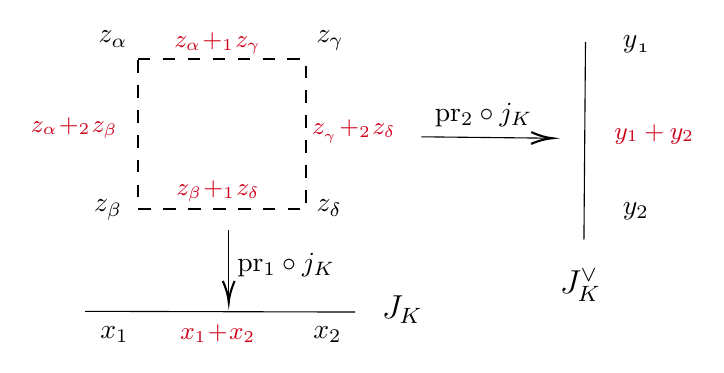
\begin{tikzpicture}[x=0.7pt,y=0.65pt,yscale=-1,xscale=1]
%Shape: Rectangle [id:dp09615503602756892] 
\draw  [dash pattern={on 4.5pt off 4.5pt}][line width=0.75]  (195.6,127.81) -- (282.39,127.81) -- (282.39,211.17) -- (195.6,211.17) -- cycle ;
%Straight Lines [id:da269614448128356] 
\draw    (168.31,267.88) -- (307.65,268.28) ;
%Straight Lines [id:da17415385155572372] 
\draw    (426.62,118.03) -- (425.81,228) ;
%Straight Lines [id:da8698879904003434] 
\draw    (242.46,222.88) -- (242.46,260.8) ;
\draw [shift={(242.46,262.8)}, rotate = 270] [color={rgb, 255:red, 0; green, 0; blue, 0 }  ][line width=0.75]    (10.93,-3.29) .. controls (6.95,-1.4) and (3.31,-0.3) .. (0,0) .. controls (3.31,0.3) and (6.95,1.4) .. (10.93,3.29)   ;
%Straight Lines [id:da09089663483493293] 
\draw    (341.88,170.86) -- (407.51,171.62) ;
\draw [shift={(409.51,171.65)}, rotate = 180.66] [color={rgb, 255:red, 0; green, 0; blue, 0 }  ][line width=0.75]    (10.93,-3.29) .. controls (6.95,-1.4) and (3.31,-0.3) .. (0,0) .. controls (3.31,0.3) and (6.95,1.4) .. (10.93,3.29)   ;

% Text Node
\draw (173.97,110.59) node [anchor=north west][inner sep=0.75pt]   [align=left] {$\displaystyle z_{\alpha }$};
% Text Node
\draw (171.62,204.52) node [anchor=north west][inner sep=0.75pt]   [align=left] {$\displaystyle z_{\beta }$};
% Text Node
\draw (286.52,204.5) node [anchor=north west][inner sep=0.75pt]   [align=left] {$\displaystyle z_{\delta }$};
% Text Node
\draw (286.43,110.5) node [anchor=north west][inner sep=0.75pt]   [align=left] {$\displaystyle z_{\gamma }$};
% Text Node
\draw (174.79,275) node [anchor=north west][inner sep=0.75pt]    {$x_{1}$};
% Text Node
\draw (284.8,275) node [anchor=north west][inner sep=0.75pt]    {$x_{2}$};
% Text Node
\draw (444.52,113.34) node [anchor=north west][inner sep=0.75pt]    {$y\mathnormal{_{1}}$};
% Text Node
\draw (444.52,205.71) node [anchor=north west][inner sep=0.75pt]    {$y_{2}$};
% Text Node
\draw (245.54,234.24) node [anchor=north west][inner sep=0.75pt]    {$\mathrm{pr_{1}} \circ j_{K}$};
% Text Node
\draw (347.47,150.91) node [anchor=north west][inner sep=0.75pt]    {$\mathrm{pr_{2}} \circ j_{K}$};
% Text Node
\draw (320.1,257.96) node [anchor=north west][inner sep=0.75pt]  [font=\large]  {$J_K$};
% Text Node
\draw (412,243) node [anchor=north west][inner sep=0.75pt]  [font=\large]  {$J_K^\vee $};
% Text Node
\draw (138.95,158.56) node [anchor=north west][inner sep=0.75pt]  [font=\small,color={rgb, 255:red, 208; green, 2; blue, 27 }  ,opacity=1 ] [align=left] {$\displaystyle z_{\alpha }\!+_{2}\! z_{\beta }$};
% Text Node
\draw (284.1,159.91) node [anchor=north west][inner sep=0.75pt]  [font=\small,color={rgb, 255:red, 208; green, 2; blue, 27 }  ,opacity=1 ] [align=left] {$\displaystyle z_{_{\gamma }}\!+_{2}\! z_{\delta }$};
% Text Node
\draw (213.02,111.59) node [anchor=north west][inner sep=0.75pt]  [font=\small,color={rgb, 255:red, 208; green, 2; blue, 27 }  ,opacity=1 ] [align=left] {$\displaystyle z_{\alpha }\!+_{1}\! z_{\gamma }$};
% Text Node
\draw (214.02,193.78) node [anchor=north west][inner sep=0.75pt]  [font=\small,color={rgb, 255:red, 208; green, 2; blue, 27 }  ,opacity=1 ] [align=left] {$\displaystyle z_{\beta }\!+_{1}\! z_{\delta }$};
% Text Node
\draw (216.11,274) node [anchor=north west][inner sep=0.75pt]  [font=\small,color={rgb, 255:red, 208; green, 2; blue, 27 }  ,opacity=1 ] [align=left] {$\displaystyle x_{1} \!+ \!x_{2}$};
% Text Node
\draw (440.2,162.47) node [anchor=north west][inner sep=0.75pt]  [font=\small,color={rgb, 255:red, 208; green, 2; blue, 27 }  ,opacity=1 ] [align=left] {$\displaystyle y_{1} +y_{2}$};
\end{tikzpicture}
}
\end{center}
Next we briefly describe the action of $\Gm$ on the Poincar\'e torsor (or more general biextensions). To this end, we let $e_{J_K}\in \Hom_{J_K}(J_K, P_K^\vee)$ (resp. $e_{J_K^\vee}\in \Hom_{J_K^\vee}(J_K^\vee, P_K^\times)$) denote the identity section of $P_K^\times$ as a $J_K$ (resp. $J_K^\vee$)-group scheme. 
  %The identity section $e_{J_K^\vee}$ induces upon pull-back via the zero section $0 : \spec K \lra J_K^\vee$ the canonical rigidification of $P_K^\times$ over $J_K \times \{ 0 \}$. Similarly, $e_{J_K}$ induces the canonical rigidification of $P_K^\times$ over $\{ 0 \}\times J_K^\vee$. These rigidifications agree over $\{ 0 \}\times \{ 0 \}$ and the group laws $+_1$ and $+_2$ agree on $P_K^\times$ over $\{ 0 \}\times \{ 0 \}$ and are given by the group law on $\G_m$ obtained by transport of structure.   
Restricting the short exact sequence (\ref{ext1}) of commutative $J_K^\vee$-group schemes via the identity section $\spec K \ra J_K^\vee $, we get a short exact sequence of commutative $K$-group schemes 
%\begin{equation}\label{diag:split}
\[\begin{tikzcd}[bend angle = 20]
1 \arrow{r}
& \G_{m, K} \arrow{r}
& P^\times_{K} \vert_{J_K\times \{ 0 \}} \arrow{r}
& J_K \arrow{r} \arrow[bend right,end anchor={[shift={(0pt,-6pt)}]}]{l}[swap]{e_{J_K}}
& 0
\end{tikzcd}\]
%\end{equation} 
which is split by the section $e_{J_K}$. In particular, we have 
$ P^\times_{K} \vert_{J_K\times \{ 0 \}}=\G_{m, J_K}$ which is $\G_{m, K}\times J_K,$ and by a similar reasoning (using the identity section $e_{J_K^\vee}$) 
$P^\times_{K} \vert_{\{ 0 \} \times J_K^\vee}=\G_{m, J_K^\vee}. $
These canonical splittings  allow for a useful description of the $\G_m$-action on $P^{\times}_K$ in terms of the partial group laws $+_2$ and $+_1$. For a $(J_K\times J_K^\vee)$-scheme $S$, consider $t \in P_K^{\times}(S)$ and $u \in \G_m(S)$ and let $(x, y)$ be the image of $t$ in $(J_K \times J_K^{\vee})(S)$. Consider a point $v=v_{x, u} \in P_K^{\times}(S)$ lying over $(x, 0)$, corresponding to $(u, 0)$ under the identification ${P_K^{\times}}\vert_{J_K \times \{0\}}(S) \simeq \G_m(S) \times J_K(S)$.\footnote{ The point $v_{x, u}$ does not depend on $t$, only on $x$ and $u$. The change of $v_{x, u}$ in the parameter $x$ is described by the relative group law $+_1,$ namely $v_{x_1+x_2, u}=v_{x_1, u}+_1v_{x_2, u}$. Similarly, we have $v_{x, u_1u_2}=v_{x, u_1}+_2v_{x, u_2}$.} 
The action of $u$ on the point $t$ is given by
\begin{equation}\label{rem:internal-Gm-action}
u \cdot t=v+_2 t.
\end{equation}
Clearly, instead of using the point $(x, 0)$, one could work with $(0, y)$ and the operation $+_1$. These two points of view are equivalent by the compatibility between $+_1$ and $+_2$. As a consequence, the $\G_m$-action commutes with the operations $+_1$ and $+_2$: given two points $a, b \in P_K^{\times}(S)$ lying over points of the form $(x, *)$ in $J_K\times J_K^{\vee}(S)$ %(so that $a+_2b$ makes sense) 
and $u, u' \in \G_m(S),$ we have
\begin{align*}
(u \cdot a)+_2(u' \cdot b)& = (v_{x, u}+_2 a)+_2(v_{x, u'}+_2 b)\\
& =(v_{x, u}+_2v_{x, u'})+_2(a+_2b) \\
%& = v_{x, uu'}+_2(a+_2b) \\
& =(uu') \cdot (a+_2b),
\end{align*}
and similarly for $+_1$.
  
 





\subsection{Spread out}\label{s:spread}

As will become apparent, in the method of geometric quadratic Chabauty it is crucial to spread out the geometry over $\oh_K$. Roughly speaking, one wants to work with finitely generated $\Z$-modules, and $\G_m(\oh_K)=\oh_K^\times$  is a finitely generated $\Z$-module of rank $\delta=r_1+r_2-1$ while $\G_m(K)=K^\times$ has infinite rank. 

Let $\CC$ denote a regular proper model of $C_K$ over $\oh_K$. Let $\CC^{\sm}$ denote the smooth locus of $\CC$. % i.e., the open subscheme consisting of points at which $C$ is smooth over $\oh_K$. 
By properness and regularity, we have the identifications 
$$    C_K(K)=\CC(\oh_K)=\CC^{\sm}(\oh_K) .$$
%where the first equality follows from properness and the second from the regularity of the model $C$.
Let $\J$ and $\J^{\vee}$ denote respectively the N\'eron models of $J_K$ and $J_K^{\vee}$ over $\oh_K$. Denote by $\J^{\circ}$ and $\Jo$ the fiberwise connected components of $0$ in $\J$ and $\J^{\vee}$ respectively. The quotient $\J/\J^{\circ}$ is an \'etale group scheme over $\oh_K$ with finite fibers. 

Suppose that $C_K(K)$ is non-empty and let $b\in C_K(K)$ be a fixed  rational point. Such a choice leads to the Abel-Jacobi map $j_b : C_K\hookrightarrow J_K$ which sends a point $x$ to the linear equivalence class of the divisor $(x)-(b)$.
The map $j_b$ extends uniquely to a morphism 
%\begin{equation}\label{map:AJOK}
   $$ j_b: \CC^{\text{sm}}\rightarrow \J $$
%\end{equation}
over $\oh_K$ by the N\'eron Mapping Property, which we shall again denote by $j_b$. Next we wish to extend the Poincare bundle to $\spec \oh_K$. As alluded to above, this is supplied by Grothendieck's theory of biextensions. 

\begin{proposition} 
The Poincar\'e torsor $P_K^{\times}$ extends uniquely to a biextension $\P^\times$ over $(\J, \Jo)$ by $\G_m$. In particular, given an $\oh_K$-scheme $S$ and two points $(x, y), (x, y') \in \J\times \Jo(S)$, we have an isomorphism 
\begin{equation}\label{isom:cube}
 (x, y)^* \P \otimes (x, y')^* \P \cong (x, y+ y')^* \P,
 \end{equation}
where $\P$ is the line bundle over $\J \times \Jo$ corresponding to $\P^\times$. 
\end{proposition} 

\begin{proof}
This is \cite[VIII. Theorem 7.1(b)]{SGA7}. Note that we have restricted to the connected subscheme $\Jo$ in order to apply the theorem cited above. 
\end{proof}

We denote the structural morphism of this $\G_m$-torsor by 
$$j : \P^{\times}\rightarrow \J\times \Jo. $$ 
The uniqueness of the extension follows from the connectedness of $\Jo$. Let us remark that the commutative group scheme extension structures and their compatibilities (from our discussion in  \S \ref{S:PoincareTorsor}) extend to the integral version $\P^\times$. 
 






\subsection{Integral points on the Poincar\'e torsor}\label{S:lifting}

The goal of this subsection is to lift certain integral points on $\J \times \Jo$ across the structure map $j: \P^\times \ra \J \times \Jo$. Let $(x, y)\in \J\times \Jo(\oh_K)$ be an $\oh_K$-point of $\J\times \Jo$, and  $(x, y)^* \P^{\times}$ be the pull-back of $\P^{\times}$ to $\oh_K$, which is a $\G_{m, \oh_K}$-torsor over $\spec \oh_K$ as shown in the diagram
\begin{equation}\label{diag:lift}
\begin{tikzcd}
(x, y)^* \P^\times\arrow{r}\arrow{d} \arrow[dr, phantom, near start, "\square"]
  & \P^\times  \arrow{d} \\
  \spec \oh_K \arrow{r}{(x, y)}
  & \J\times  \Jo.
\end{tikzcd}
\end{equation}
Lifting the point $(x, y)$ to $\P^\times$ amounts to finding a section of the torsor $(x, y)^* \P^\times \ra \spec \oh_K$. 

Note that, in the case $K=\Q$, all $\Gm$-torsors are trivial over $\spec \Z$ and admit a section over $\Z$, unique up to $\G_m(\Z)=\{ \pm 1 \}$. Thus a lift of the integral point $(x, y)$ to $\P^\times$ always exits. 
%\begin{tikzcd}[bend angle = 20] (x, y)^* P^\times\arrow{r}\arrow{d}   & P^\times  \arrow{d} \\   \spec \Z \arrow[bend left]{u}{s} \arrow{r}{(x, y)} \arrow[dashrightarrow]{ru}    & J\times J^{\vee, 0}. \end{tikzcd}
 In the case of a general number field $K$, it is not always possible to lift an $\oh_K$-point $(x, y)$ of $\J\times \Jo$ to $\P^\times$ when the class number $h$ of $K$ is non-trivial. However, the previous argument carries over to $\oh_K$-points of the form $(x, h\cdot y)$. More precisely, we have 

\begin{lemma}\label{lem:h}
Any $\oh_K$-point of $\J\times \Jo$ of the form $(x, h\cdot y)$ where $(x, y)\in \J\times \Jo (\oh_K)$ admits a lift to an $\oh_K$-point of the Poincar\'e torsor $\P^\times$. This lift is unique up to multiplication by an element of $\oh_K^\times$.
\end{lemma}

\begin{proof}
We repeatedly apply the isomorphisms (\ref{isom:cube}) % in the case $S=\spec \oh_K$ with $x\in J(\oh_K), y\in J^{\vee, 0}(\oh_K)$ and $y'=n\cdot y\in J^{\vee, 0}(\oh_K)$ with $n=1, \ldots, h-1$. In this way we obtain an isomorphism of $\G_{m, \oh_K}$-torsors over $\oh_K$
and obtain an isomorphism
$$
    ((x, y)^* \P)^{\otimes h} \cong (x, h\cdot y)^* \P
$$
of line bundles over $\spec \oh_K$. In particular, we know that $(x, h\cdot y)^* \P^\times$ is trivial as a $\G_m$-torsor over $\oh_K$, since $\Pic (\oh_K)$ has size $h$. 
\end{proof}



\subsection{Trivialization of the Poincar\'e torsor} \label{trivialization}




%\subsection{Trivializing the Poincar\'e torsor over the curve}

Next we define and study a certain $\G_m^{\rho-1}$-torsor $\TT$ over $\J$, where $\rho$ is the rank of the N\'eron--Severi group of $J_K$. The goal of this subsection is to lift the Abel-Jacobi map $j_b: \CC^{\textup{sm}} \ra \J$ across $\TT \ra \J$. As discussed in the introduction, this is a crucial step in the geometric approach to quadratic Chabauty. 

\subsubsection{Trivialization over $C_K$}

Let  $\lambda : J_K\lra J_K^\vee$ be the canonical principal polarization. By functoriality of $\Pic$ we have the following commutative diagram of commutative $K$-group schemes with exact rows: 
\begin{equation}\label{diag:NS}
\begin{tikzcd}[bend angle = 20]
  0 \arrow{r}
  & J_K^\vee \arrow{r} \arrow{d}{-\lambda^{-1}}[swap]{\wr}
  & \Pic_{J_K/K} \arrow{r}{\pi} \arrow{d}{j_b^*}
  & \NS_{J_K/K} \arrow{r} \arrow{d}{j_{b, \NS}^*}
  & 0 \\
  0 \arrow{r}
  & J_K \arrow{r}
  & \Pic_{C_K/K} \arrow{r}{\deg}
  & \Z_K \arrow{r}
  & 0.
\end{tikzcd}
\end{equation}
Here $\NS_{J_K/K}$ denotes the N\'eron--Severi group scheme of $J_K$, i.e., the \'etale $K$-group scheme of components of the Picard scheme associated to $J_K$. Here we have used the fact that the map induced by $j_b$ on $\Pic^0$ agrees with $-\lambda^{-1}$, which is in particular an isomorphism. 

Next, let $\Hombf(J_K, J_K^\vee)^{+} \subset \Hombf(J_K, J_K^\vee)$ denote the closed subgroup scheme of self-dual homomorphisms (see \cite[Proposition 7.14 \& \S 7.18]{EGM} for representability). There is a map 
$$
    \varphi : \Pic_{J_K/K}\lra \Hombf(J_K, J_K^\vee)^+ %\qquad [\sL]\mapsto \varphi_{\sL}
$$
defined by sending the class of a line bundle $L$ to the map $\varphi_L$, which maps a closed point $x\in J_K \mapsto  [\tr_x^* L\otimes L^{-1}]$ where $\tr_x : J_K\lra J_K$ denotes translation by $x$. The kernel of $\varphi$ is equal to $\Pic^0_{J_K/K}=J_K^\vee$ and the map $\varphi$ induces an isomorphism of $K$-group schemes \cite[Corollary 11.3]{EGM}
\begin{equation}\label{map:phitilde}
    \tilde{\varphi} : \NS_{J_K/K}\overset{\sim}{\lra} \Hombf(J_K, J_K^\vee)^+.
\end{equation}

\begin{definition} 
At the level of $K$-points, we define the group $\Hom(J_K, J_K^\vee)_0^+$ to be the kernel 
$$
\Hom(J_K, J_K^\vee)_0^+ := \ker \left( j_{b, \NS}^*\circ \tilde{\varphi}^{-1}: \Hom(J_K, J_K^\vee)^+ \ra \Z \right) 
$$ %(which is equal to minus the trace of $\lambda^{-1}\circ 2f$ acting on $H_1(J_K(\C), \Z)$).
\end{definition}

\begin{proposition}\label{prop:trivtorsor}
For all $f\in \Hom(J_K, J_K^\vee)_0^+$, there exists a unique element $c_f\in J_K^\vee(K)$ with the property that the following $\G_m$-torsor over $C_K$
$$
j_b^*(\id, \tr_{c_f}\circ f)^* P_K^\times
$$ 
is trivial. Here $(\id, \tr_{c_f} \circ f)$ denotes the map $J_K \xrightarrow{(\id, \tr_{c_f} \circ f)} J_K \times J_K^\vee$. 
In particular, for all $n\in\Z_{\ge 1}$, its $n^\text{th}$ power $j_b^*(\id, n\cdot \circ \tr_{c_f}\circ f)^* P_K^\times$ is also trivial. 
\end{proposition}

\begin{proof}
At the level of $\overline{ K}$-points, the diagram (\ref{diag:NS}) can be written as follows: 
\begin{equation}\label{diag:NSK}
\begin{tikzcd}[bend angle = 20]
%0 \arrow{r}
%  & 0  \arrow{r} \arrow[hook]{d}
& & &  \Hom(J_K, J_K^\vee)_0^+ \arrow[d, hook] \arrow[ddl, dashed, bend right, start anchor={[shift={(0pt,-3pt)}]}, end anchor={[shift={(3pt,0pt)}]}, near start, "s_1"] \arrow[ddl, dashed, bend right, swap, near start, "s_2"] \\
&  & \ker (j_{b,\overline{ K}}^*) \arrow[r, swap, "\sim"] \arrow[hook]{d}
  & \ker (j_{b, \overline{K}, \NS}^*) \arrow[hook]{d} %\arrow{r}   & 0 
\\
  0 \arrow{r}
  & J_K^\vee(\overline{K}) \arrow{r} \arrow{d}{-\lambda^{-1}}[swap]{\wr}
  & \Pic(J_{\overline{K}}) \arrow{r}{\pi} \arrow{d}{j_{b, \overline{K}}^*}
  & \NS_{J_K/K}(\overline{K}) \arrow{r} \arrow{d}{j_{b,\overline{K}, \NS}^*}
  & 0 \\
  0 \arrow{r}
  & J_K(\overline{K}) \arrow{r}
  & \Pic(C_{\overline{K}}) \arrow{r}{\deg}
  & \Z \arrow{r}
  & 0.
\end{tikzcd}
\end{equation}
%The fact that $\lambda$ is an isomorphism implies, by the Snake Lemma, that the top row is exact.
The map $\pi$ in the first  short exact sequence in this diagram admits two splittings when restricted to $ \Hom(J_K, J_K^\vee)_0^+$, which is viewed as a subgroup of $\ker (j_{b, \overline{K}, \NS}^*)$ via $\tilde \varphi^{-1}$. The first section 
 $$s_1 : \Hom(J_K, J_K^\vee)^+ \lra \Pic(J_{\overline K})$$
  is defined by mapping a self-dual homomorphism $f$ (defined over $K$) to the isomorphism class of the $\G_m$-torsor $L_f^\times:=(\id, f)^* P_K^\times$ on $J_K$, which is an element in $\Pic (J_K) \subset \Pic (J_{\overline{K}})$. 
We observe that  (\cite[Proposition 11.1]{EGM})
$$
\tilde{\varphi}\circ \pi \circ s_1(f)=\varphi_{L_f}=f+f^\vee=2f. 
$$
 The second splitting is given by inverting $\pi$ on $\ker (j_{b, \overline{K}}^*)$, in other words, by 
 $$
s_2 :\Hom(J_K, J_K^\vee)_0^+  \hookrightarrow \ker (j_{b, \overline{K}, \NS}^*)  \overset{\pi^{-1}}{\lra} \ker (j_{b, \overline{K}}^*) \subset \Pic(J_{\overline{K}}).$$
Again the image of $s_2$  lies in $\Pic(J_K).$ Now, given $f\in \Hom(J_K, J_K^\vee)_0^+$ we define 
$$
c_f:=2s_2(f)-s_1(f)\in \Pic (J_K).
$$
As $ c_f \in \ker (\pi)$ we thus have $c_f \in J_K^{\vee} (K)$. Now we observe that, for a line bundle $L$ on $J_K$ corresponding to a closed point $x \in J_K^\vee$,  we have
$$(\id, f)^* P_K \otimes L \cong (\id, f)^* \big( P_K \otimes \textup{pr}_1^* L \big) \cong (\id, f)^* \Big( (\id \times \tr_{x})^* P_K  \Big),$$
where $\textup{pr}_1$ is the projection $J_K \times J_K^\vee \ra J_K$. 
Therefore, by construction, $c_f$ is the unique element in $J_K^\vee(K)$ such that
$$
s_1(f)+c_f=[(\id, \tr_{c_f}\circ f)^* P_K^\times]\in \ker j_{b}^*.
$$
This proves the proposition. 
\end{proof}


The group $\NS_{J_K/K}(K)$ is a finitely generated free $\Z$-module whose rank is denote by $\rho$ (the Picard number of $J_K$). The kernel 
$$\ker (j_{b, \NS}^*: \NS_{J_K/K} (K) \ra \Z)$$ is a free $\Z$-module of rank $\rho-1$, and so is the group $\Hom(J_K, J_K^\vee)_0^+$.

\begin{notation} \label{notation:f_i} 
We fix the following notations from now on.
\begin{itemize} 
\item Let $f_1, \ldots, f_{\rho-1}$ be a basis of $\Hom(J_K, J_K^\vee)_0^+$. 
\item For each $i=1, \ldots, \rho-1$, let $c_i:=c_{f_i}\in J_K^\vee(K)$ be the element corresponding to $f_i$ in Proposition \ref{prop:trivtorsor}.
\item For each integer $n\in \mathbb{Z}_{\ge 1}$, denote by $\alpha_{n, i, K}$ the map 
$$
\alpha_{n, i, K}: J_K \xrightarrow{(\id, n\cdot \circ \tr_{c_i} \circ f_i)} J_K\times J_K^\vee.
$$
\end{itemize}
\end{notation}

\begin{construction}\label{cons:lifting_over_K} By Proposition \ref{prop:trivtorsor}, the pull-back $j_b^* \big( \alpha_{n, i, K}^* P_K^\times \big)$ is a trivial $\G_m$-torsor over $C_K$. 
In particular, it admits a section over $C_K$. This gives rise to a lift of $j_b$, which we shall fix and denote by $\tilde{j}_{b}^{(n, i)}$ as in the diagram below.  This choice is unique up to $K^\times$.
\begin{equation}\label{diag:AJliftK}
\begin{tikzcd}[bend angle = 20]
  & \alpha_{n, i, K}^* P_K^\times  \arrow{r} \arrow{d} \arrow[phantom]{dr}{\square}
  & P_K^\times \arrow{d} \\
  C_K \arrow{r}{j_b} \arrow[dashrightarrow]{ru}{\tilde{j}_{b}^{(n, i)}}
  & J_K \arrow{r}{\alpha_{n, i, K}}
  & J_K\times J_K^\vee.
\end{tikzcd}
\end{equation}
\end{construction}

 

\subsubsection{Construction over $\oh_K$}

Now we extend the geometry over $\oh_K$. Let us introduce and recall some notations and refer the rest to $\S \ref{s:spread}$. Let $\mathfrak{n}$ be the product of prime ideals in $\oh_K$ such that $\CC$ is smooth away from $\spec(\oh_K/\mathfrak{n})$. Let $\Phi^\vee = \J^\vee / \Jo$ be the group scheme of connected components of $\J^\vee$. It is trivial outside $\oh_K/\mathfrak{n}$ with finite \'etale fibers over $\oh_K/\mathfrak{n}$. Let $m$ denote the least common multiple of the exponents of $\Phi^\vee(\bar{\F}_\mathfrak{q})$ over all prime ideals $\mathfrak{q}$ of $\oh_K$. Finally, recall that $h$ denotes the class number of $K$. 

By the N\'eron mapping property, for each $1\leq i\leq \rho-1$, the homomorphism $f_i : J_K\lra J_K^\vee$ (resp. the translation map $\tr_{c_i} : J_K^\vee \lra J_K^\vee$, resp.  the multiplication $hm\cdot : J_K^\vee \lra J_K^\vee$) extends uniquely to a homomorphism  $f_i : \J\lra \J^\vee$ (resp.  $\tr_{c_i} : \J^\vee \lra \J^\vee$, resp.  $hm\cdot : \J^\vee \lra \J^\vee$).  Note that $c_i\in J_K^\vee(K) =  \J^\vee(\oh_K)$. Therefore, the morphism $\alpha_{hm, i, K} : J_K\lra J_K\times J_K^\vee$ extends uniquely to a morphism of $\oh_K$-schemes 
$$\alpha_{hm, i} = (\id, hm\cdot \circ \tr_{c_i} \circ f_i): \J\lra  \J\times \J^\vee.$$  
The integer $m$ is chosen so that the image of this map lies in $\J\times \Jo$. 

\begin{construction} \label{map:alpha} 
Taking the product over $i=1, \ldots, \rho-1$, we obtain the $\oh_K$-morphism
\begin{align*} 
    \alpha & =(\id, ({hm\cdot} \circ \tr_{\underline{c}} \circ \underline{f})) \\
    & :=(\id, ({hm\cdot} \circ \tr_{c_i} \circ f_i)_{i=1}^{\rho-1}) : \J \lra \J\times (\Jo)^{\rho-1}
\end{align*}
Consider the map $\P^\times \rightarrow \J \times \Jo \rightarrow \J$ defined as the composition of the structure map $j$ with the first projection. Using this morphism, we form the $(\rho-1)$-fold self-product 
$$
    \P^{\times, \rho-1}:= \P^\times \times_{\J} \ldots \times_{\J} \P^\times.
$$
We naturally have a morphism
$    \P^{\times, \rho-1} \lra \J\times (\Jo)^{\rho-1},$
which endows $\P^{\times, \rho-1}$ with the structure of a $\G_m^{\rho-1}$-torsor over $\J\times (\Jo)^{\rho-1}$.
\end{construction}
 

This leads to the following key construction in the article. 
\begin{definition}Retain notations from Construction \ref{map:alpha}. We define the $\G_m^{\rho-1}$-torsor $\TT$ over $\J$ to be the pull-back of the $\G_m^{\rho-1}$-torsor $\P^{\times, \rho-1}$ over $\J\times (\Jo)^{\rho-1}$ by the map $\alpha$:
\begin{align*}
    \TT:= & \P^{\times, \rho-1}\times_{\alpha} \J=\alpha^* \P^{\times, \rho-1} \\ = &
    (\id, hm\cdot \circ \tr_{c_1} \circ f_1)^* \P^\times\times_{\J} \ldots \times_{\J}(\id, hm\cdot \circ \tr_{c_{\rho-1}} \circ f_{\rho-1})^* \P^\times.
\end{align*}
\end{definition}

\begin{construction} Now we return to the lifts $\tilde{j}_b^{(hm, i)}$ obtained in Construction \ref{cons:lifting_over_K}. By taking the product over $i$ of these lifts $\tilde{j}_b^{(hm, i)}$, we obtain a lift $\tilde{j}_b$ of $j_b$ to $T_K:=T\times_J J_K$ as pictured in the following commutative diagram:
\begin{equation}\label{diag:AJliftTK}
\begin{tikzcd}[bend angle = 20]
  & T_K  \arrow{r} \arrow{d} \arrow[phantom]{dr}{\square}
  & P_K^{\times, \rho-1} \arrow{d} \\
  C_K \arrow{r}{j_b} \arrow[dashrightarrow]{ru}{\tilde{j}_{b}}
  & J_K \arrow{r}{\alpha_K}
  & J_K\times (J_K^{\vee, 0})^{\rho-1}
\end{tikzcd}
\end{equation}
where $\alpha_K$ denotes the base change of the map $\alpha$  to $K$.
\end{construction}


Our goal is to extend this diagram over $\oh_K$. However, lifting the map $j_b : \CC^{\sm}\lra \J$ to the torsor $\TT$ is not generally possible: the problem is that, for primes $\mathfrak{q}\vert \mathfrak{n}$, the fiber $C^{\sm}_{\F_\mathfrak{q}} := \CC^{\sm} \times_{\spec \oh_K} \spec {\F_{\mathfrak{q}}}$ may contain too many components. To remedy this, we consider one geometrically irreducible component in each such fiber at a time.  

\begin{construction} \label{cons:U}
Let $\U \subset \CC^{\sm}$ be an open subscheme obtained by removing, for every $\mathfrak{q} \vert \mathfrak{n}$, all but one irreducible component of $C^{\sm}_{\F_\mathfrak{q}}$ that is further geometrically irreducible. We will later lift the map $j_b$ to a map $\tilde j_b^U: \U \lra \TT$ for each such open subscheme $\U$.   
\end{construction}

\begin{remark}\label{remark:U} We first remark that  such a subscheme $\U$ exists under the assumption that $C_K$ admits a $K$-rational point. Moreover, for our purposes of determining the set of rational points $C_K (K) = \CC^{\sm} (\oh_K)$, it suffices to consider subschemes of the form $\U$ as there are finitely many of them and each point in $\CC^{\sm}(\oh_K)$ lies in exactly one such $\U$. Both remarks follow from the following simple lemma. 
\end{remark}

\begin{lemma}
Let $X$ be a smooth irreducible affine curve over a finite field $k$ that admits a $k$-rational point, then $X$ is geometrically irreducible. 
\end{lemma}
 
%The claim is standard. Find a reference and delete the proof... %Surely this can be found in EGA somewhere... 
 
\begin{proof} Let $A = \Gamma(X, \oh_X)$ be the ring of sections on $X$, which  admits a map $A \rightarrow k$ of $k$-algebras supplied by the rational point. Let $k' = \{\alpha \in k(X) | \alpha \textup{ is algebraic over } k\}$ be field of constants of $X$ over $k$, as $X$ is normal we have $k' \subset A$ which forces $k' = k$. This is equivalent to $X$ being geometrically irreducible. 
\end{proof}


\subsubsection{The lift to $\TT$} 

We are finally able to construct the desired lift of $j_b$. Our construction is  analogous to that in \cite[\S 2]{EL19} except that we pull back $\P^{\times}$ via morphisms of the form $(\id, {hm\cdot}\circ \tr_c\circ f):\J\rightarrow \J\times \Jo$, where in the second factor we incorporate an additional multiplication by $h$ (the class number of $\oh_K$), to ensure the existence of such a lift.

\begin{proposition}\label{prop:Ulift}
Let $\U$ be an open subscheme of $\CC^{\sm}$ obtained as in Construction \ref{cons:U}. Then there exists a lift $\tilde{j}_b^U$ of $j_{b}\vert_{\U}$ to $\TT$, unique up to $\oh_K^{\times, \rho-1}$, which makes the following diagram commute:
\begin{equation}\label{diag:AJliftU}
\begin{tikzcd}[bend angle = 20]
  &
  & \TT  \arrow{r} \arrow{d} \arrow[phantom]{dr}{\square}
  & \P^{\times, \rho-1} \arrow{d} \\
  \U \arrow[hook]{r} \arrow[dashrightarrow]{rru}{\tilde{j}_{b}^U}
  & \CC^{\sm} \arrow{r}{j_b} 
  & \J \arrow{r}{\alpha}
  & \J\times (\Jo)^{\rho-1}.
\end{tikzcd}
\end{equation}
\end{proposition}

\begin{proof}
The restriction of the torsor
$$(\id, m\cdot \tr_{c_i} \circ f_i)^* \P^\times$$ to $\U$ gives an element of $\Pic(\U)$, whose pull-back to $C_K$ equals 
$$j_{b}^*\alpha_{m, i, K}^*P_K^{\times}$$ and is trivial by Proposition \ref{prop:trivtorsor}. In other words, the torsor $(\id, m\cdot \circ \tr_{c_i} \circ f_i)^* \P^\times$  when restricted to $\U$ gives rise to an element in the kernel 
$$\ker (\Pic (\U) \lra \Pic (C_K)).$$
Now note that we have an isomorphism of line bundles (corresponding to $\G_{m, \J}$-torsors)  
\begin{equation}
    (\id, hm\cdot \circ \tr_{c_i} \circ f_i)^*\P  \simeq ((\id, m\cdot \circ \tr_{c_i} \circ f_i)^* \P)^{\otimes h}
\end{equation}
using equation \ref{isom:cube}. By Lemma \ref{lem:PicU} below, we conclude that $(\id, hm\cdot \circ \tr_{c_i} \circ f_i)^* \P^\times$ becomes a trivial $\G_{m, \U}$-torsor when restricted to $\U$. Therefore, $\TT$ pulls back to the trivial $\G_{m, \U}^{\rho-1}$-torsor over $\U$. In particular, the map $j_b\vert_{\U}$ admits a lift to $\TT$, which is unique up to $\G_m^{\rho-1}(\U)=(\oh_\U(\U)^\times)^{\rho-1}=(\oh_K^{\times})^{\rho-1}$ again by Lemma \ref{lem:PicU}. 
\end{proof}
 
The following lemma is used in the proof above. 

\begin{lemma}\label{lem:PicU}
Let $\U$ be an open subscheme of $\CC^{\sm}$ as above. Then $\oh_{\U}(\U)=\oh_K$ and the kernel of the restriction $\ker(\Pic(\U)\lra  \Pic(C_K))$ is entirely $h$-torsion. In other words, for a line bundle $L$ over $\U$ that becomes trivial over the generic fiber $C_K$, $L^{\otimes h}$ is trivial over $\U$. 
%$$\left\{hx \vert x \in \Pic(\U), x \mapsto 0 \in \Pic(C_K) \right\}  = 0.$$
\end{lemma}

\begin{proof}
By construction $\U$ is regular thus locally factorial, so we do not distinguish the class of line bundles and Weil divisors.  First let $D$ be a vertical divisor on $\U$, namely it does not intersect the generic fiber $C_K$. We claim that $h D = 0$ in $\Pic (\U)$. As every irreducible vertical divisor on $\U$ is of the form $\U_\mathfrak{p}$ for some prime $\mathfrak{p}$ of $\oh_K$,  we may write $h D$ as 
$\sum_{\mathfrak{p}} h n_\mathfrak{p} U_{\F_\mathfrak{p}},$ where $n_{\mathfrak{p}}=0$ for almost all $\mathfrak{p}$. Clearly $D$ is the image of the divisor $\sum_{\mathfrak{p}} h n_{\mathfrak p}$ along the natural map $\Pic (\oh_K) \ra \Pic (\U)$, which is $0$ since $\Pic (\oh_K)$ has size $h$. Now let $D$ be a general element of $\Pic(\U)$ (which we view as a Weil divisor on $\U)$ that lies in the kernel $\ker (\Pic (\U) \rightarrow \Pic (C_K))$. In other words, the restriction of $D$ to $C_K$ is a principal divisor $D_K = \textup{div} (f)$ for some $f$ in the function field of $C_K$. Then $\textup{div} (f)$ extends to a principal divisor on $\U$, which differs from $D$ only by a vertical divisor. The lemma thus follows.  
\end{proof}

\begin{remark}
When $h = 1$ the lemma simply says that the restriction $\Pic (\U) \rightarrow \Pic (C_K) $ is injective. This map is of course not in general injective when $h\neq 1$.  Indeed, in the case it suffices to take $D=U_{\mathfrak{p}}\in \Div(\U)$ where $\mathfrak{p}$ is a non-principal prime ideal of $\oh_K$.  
\end{remark}




%%%
%%%
%%%
%%%
%%%
%%% 

\section{The main theorem}\label{s:method}

In this section we state the main theoretical results of the paper. We  also describe the strategy of the geometric method in slightly more detail. 

\begin{assumption}\label{passumption} 
 Throughout, we make the following assumption on the prime $p$. 
\begin{itemize}
\item The curve $C_K$ has good reduction at each prime $\mathfrak{p}_1, \ldots, \mathfrak{p}_s$ of $K$ that sits above $p$. 
\item Each $\mathfrak{p}_i$ satisfies $e(\mathfrak{p}_i/p) < p-1$. 
\item Finally, $p$ does not divide $\vert \oh_{K, \mathrm{tors}}^\times \vert$.
\end{itemize}
\end{assumption}
\noindent Note that the first condition is equivalent to requiring that $\mathfrak{p}_i \nmid \mathfrak{n}$ for each $1\leq i\leq s$. %Moreover, the condition $e(\mathfrak{p}/p)<p-1$ forces $p>2$. 
The set of primes $p$ satisfying Assumption \ref{passumption} clearly has positive density. 

%Let therefore $p$ denote the choice of a rational odd prime. Throughout, we will make the following assumption:
%\begin{assumption}\label{passumption}
%The prime $p$ is either unramified in $K$ or satisfies $p>[K:\Q]$. It does not divide $\vert \oh_{K, \tors}^\times \vert$. Additionally, $C$ admits good reduction at all primes of $K$ above $p$.
%\end{assumption}

\begin{notation} \label{OKp-OKP-points}
We further adopt the following notation: 
\begin{itemize}
    \item Let $\oh_{K, p}:= \oh_{K}\otimes \Z_p$ be the $p$-adic completion of $\oh_K$. % by the Chinese Remainder Theorem, it 
    This is isomorphic to the product of $\mathfrak{p}_i$-adic completions $ \oh_{K,\mathfrak{p}_1} \times \ldots \times \oh_{K,\mathfrak{p}_s}.$
    \item $\overline{\oh_{K,p}}$ denotes $(\oh_K \otimes \mathbb{F}_p)_{\mathrm{red}}$, which is isomorphic to the product of the residue fields ${ \mathbb{F}_{\mathfrak{p}_1}\times \ldots \times \mathbb{F}_{\mathfrak{p}_s}}.$
    \item   For any $\oh_K$-scheme $X$, we have natural identifications
    \begin{align*}
    X(\oh_{K, p}) &= X_{\oh_{K,\mathfrak{p}_1}}(\oh_{K,\mathfrak{p}_1}) \times \ldots \times X_{\oh_{K,\mathfrak{p}_s}}(\oh_{K,\mathfrak{p}_s}), \\
    X(\overline{\oh_{K, p}}) & =  X_{\F_{\mathfrak{p}_1}}(\F_{\mathfrak{p}_1}) \times \ldots \times X_{\F_{\mathfrak{p}_s}}(\F_{\mathfrak{p}_s}).
    \end{align*}
    We denote the natural reduction map by 
    $$ \textup{red}: X(\oh_{K, p})\lra X(\overline{\oh_{K, p}}).$$  
   \item     Given a point $x\in X(\overline{\oh_{K, p}})$, we denote by $X(\oh_{K, p})_x$ the set $\textup{red}^{-1} (x)$, 
  namely the residue disk in $X(\oh_{K, p})$ that reduces to the point $x$. Likewise, we denote by $X(\oh_K)_x$ the pre-image of $X(\oh_{K, p})_x$ under the natural inclusion 
  $$ X(\oh_K) \longhookrightarrow X(\oh_{K, p}),$$
  which consists of rational points in the residue disk $X(\oh_{K, p})_x$. 
      \end{itemize}
 \end{notation}
   
 \begin{remark} \label{remark: all_primes}
The reason to consider $\oh_{K, p}$ (instead of $\oh_{K, \mathfrak p}$ for a prime $\mathfrak p$ of $K$) is that we choose to work with all primes above $p$ simultaneously (instead of fixing a single prime) in this article. This is in agreement with the approach in \cite{siksek}.  
 \end{remark}   
  

\subsection{Revisiting the strategy}
Let $\U$ be an open subscheme of $\CC^{\sm}$ obtained in Construction \ref{cons:U}. Let $u$ be an element in the finite set $\U(\overline{\oh_{K, p}})$, and let
$$t:=\tilde{j}_b^{U}(u)\in \TT(\overline{\oh_{K, p}})$$ 
be its image in $\TT$. Note that $\CC^{\sm}(\oh_K)$ is the disjoint union of $\U(\oh_K)$ for the finitely many choices of $\U$'s (Remark \ref{remark:U}), and each $\U(\oh_K)$ is the disjoint union of finitely many ``residue disks" $\U(\oh_K)_u$. Thus, for our purposes, it suffices to bound the size $\U(\oh_K)_u$ for each $\U$ and each point $u \in \U(\overline{\oh_{K, p}})$.  
%There is a natural map $U(\oh_K)\lra U(\oh_{K,p})$ arising from the inclusions $\oh_K\hookrightarrow \oh_{K, \mathfrak{p}_i}$. Let $U(\oh_K)_u$ denote the preimage under this map of $U(\oh_{K, p})_u$. 


The key idea of the approach can be represented by the following commutative diagram:
\begin{equation}\label{diag:chab}
%\begin{tikzcd}
  % \U(\oh_K)_u \arrow[hook]{r}{\tilde{j}_b^U}  
   %\arrow[hook]{dd}
   % & \TT(\oh_K)_t \arrow[hook]{d} \\
   % &  \Y_t \arrow[hook]{d} \\
   % \U(\oh_{K, p})_u \arrow[hook]{r}{\tilde{j}_b^U} 
    %& \TT(\oh_{K, p})_t
%\end{tikzcd}
\begin{tikzcd}[row sep = 2em]
   \U(\oh_K)_u \arrow[hook]{d}{\tilde{j}_b^U}  
   \arrow[hook]{rr}
&&       \U(\oh_{K, p})_u \arrow[hook]{d}{\tilde{j}_b^U} 
 \\
   \TT(\oh_K)_t \arrow[hook]{r} 
    &  \Y_t \arrow[hook]{r} 
    & \TT(\oh_{K, p})_t
\end{tikzcd}
\end{equation}
where the top horizontal arrow is induced by the inclusion $\oh_K \hookrightarrow \oh_{K, p}$, while 
$$\Y_t := \overline{\TT(\oh_K)_t}^p$$ denotes the $p$-adic completion of $\TT(\oh_K)_t$ in $\TT(\oh_{K, p})_t$. We view $\U(\oh_K)_u$ (resp. $\U(\oh_{K, p})_u$) as a subset of $\TT(\oh_K)_t$ (resp. $\TT(\oh_{K, p})_t$) via the map $\tilde{j}_b^U$ in the diagram above. In particular, we have inclusions
$\U(\oh_K)_u \hookrightarrow   \U(\oh_{K, p})_u \cap \Y_t. $
As explained in the introduction,  our goal is to bound the intersection 
    \begin{equation}\label{intersection}
     \U(\oh_{K, p})_u \cap \Y_t
    \end{equation}
    which takes place in the $p$-adic manifold $\TT(\oh_{K, p})_t$. 
 

\begin{remark}
    For this intersection to have a chance to be finite, some conditions must be imposed in the style of the original Chabauty condition  ``$r<g$". We will come back to this point in \S \ref{s:chabcondition} after stating the main technical result of the paper. 
\end{remark}


\subsection{The key technical result}\label{s:strategy} 

In this subsection we give a description of $\Y_t$, which is a crucial step in bounding the intersection in \ref{intersection}. 
\begin{notation} \label{notation:main_thm_sec} We fix the following notations. 
\begin{itemize} 
\item Let $r:=\rank_\Z J_K(K)$ be the Mordell--Weil rank of $J_K$ over $K$. 
\item  %By the N\'eron Mapping Property we may identify the Mordell--Weil group $J_K(K)$ with $J(\oh_K)$. Let 
We let $\J(\oh_K)_0$ denote the subgroup of $J_K(K) = \J(\oh_K)$, given by kernel 
$$ \J(\oh_K)_0 := \ker \big( \textup{red}: \J(\oh_K) \rightarrow \J(\overline{\oh_{K, p}}) \big).$$ 
\item 
Let $q^*$ denote the exponent of $\G_m(\overline{\oh_{K, p}})$, that is, the least common multiple of $$q_i-1=\# \mathbb{F}_{\mathfrak{p}_i}-1$$ for $i=1, 2, \ldots, s$.
\item 
For each $i$, let $k_i = k_{\mathfrak{p}_i}=e_{\mathfrak{p}_i}f_{\mathfrak{p}_i}$ be the $\Z_p$ rank of $\oh_{K, \mathfrak{p}_i}$. Note that the rank of $\oh_{K, p}$ as a $\Z_p$-module is $\sum_{\mathfrak{p_i}\vert p} k_i =d$. 
\end{itemize}
\end{notation}


 By Assumption \ref{passumption} on $p$, we know that for each $i$, the reduction map 
$$\J(\oh_K)\rightarrow \J(\F_{\mathfrak{p}_i})$$ is injective on the torsion points of $\J(\oh_K)$ by \cite[Appendix]{katz1980galois}. Hence $\J(\oh_K)_0$ is a free $\Z$-module of rank $r$. The scheme $\TT\times_{\oh_K} \spec \oh_{K, \mathfrak{p}}$ is smooth over $\oh_{K, \mathfrak{p}}\simeq \Z_p^{k_{\mathfrak{p}}}$ of relative dimension $g+\rho-1$. By choosing a regular system of parameters for the residue disk above the point $t\in \TT(\F_\mathfrak{p})$, we obtain a homeomorphism 
$$\TT(\oh_{K, \mathfrak{p}})_t\simeq \Z_p^{(g+\rho-1)k_{\mathfrak{p}}}.$$ In particular, the dimension of $\TT(\oh_{K, p})$ as a locally analytic $p$-adic manifold is $$(g+\rho-1)\sum_{\mathfrak{p}\vert p} k_{\mathfrak{p}}=(g+\rho-1)d.$$ 

The idea is to parametrize the $p$-adic closure $\Y_t = \overline{\TT(\oh_K)_t}^p$ using the free $\Z_p$-module
\[
(\G_m^{\rho-1}(\oh_K)_{\tf} \times \J(\oh_K)_0)\otimes \Z_p.
\]
Here the subscript ``$\tf$" stands for the torsion free part. In \S \ref{s:construct}, we will prove the following proposition (in a precise form, see Proposition \ref{prop:modify-E-by-local-units}).
\begin{proposition}[Coordinates on $\TT$: rough form] \label{prop:pinterpolation}
There exists a map
\begin{equation}
    E' : \Z^{\delta(\rho-1)+r} \lra \TT(\oh_{K, p})_t
\end{equation}
(upon fixing a basis for the free $\Z$-module $\G_m^{\rho-1}(\oh_K)_{\tf} \times \J(\oh_K)_0$) which can be described using the partial composition laws described in \S \ref{S:PoincareTorsor}, and satisfies the following property 
\begin{equation}\label{eq:Eprop}
    E'(q^* \Z^{\delta(\rho-1)+r})\subset \TT(\oh_K)_t \subset E'(\Z^{\delta(\rho-1)+r}).
\end{equation}
Here $q^*$ is the integer defined in Notation \ref{notation:main_thm_sec}. 
\end{proposition}

We then $p$-adically interpolate the map $E'$ to get the following  result in \S \ref{s:interpolation}.
\begin{theorem}[$p$-adic interpolation: rough form]\label{thm:pinterpolation}
There is a unique map 
$$\kappa:  (\G_m^{\rho-1}(\oh_K)_{\tf} \times \J(\oh_K)_0)\otimes \Z_p  \: \lra \:  \TT (\oh_{K, p})_t  $$
 which makes the diagram
\[
\begin{tikzcd}[column sep = 1.2em]
\Z^{\delta(\rho-1)+r} \arrow{r}{\simeq} \arrow[hook]{d}
& \G_m^{\rho-1}(\oh_K)_{\tf} \times \J(\oh_K)_0 \arrow{rrr}{E'} \arrow[hook]{d}
&&& \TT(\oh_{K, p})_t \arrow{r}{\simeq} \arrow[equal]{d}
& \Z_p^{(g+\rho-1)d} \arrow[equal]{d} \\
\Z_p^{\delta(\rho-1)+r} \arrow{r}{\simeq}
& (\G_m^{\rho-1}(\oh_K)_{\tf} \times \J(\oh_K)_0)\otimes \Z_p \arrow[dashed]{rrr}{\exists ! \kappa} 
&&& \TT(\oh_{K, p})_t \arrow{r}{\simeq}
& \Z_p^{(g+\rho-1)d}
\end{tikzcd}
\]
commute, such that the composed map in the bottom row is given by a $(g+\rho-1)d$-tuple of convergent power series $(\kappa_1, \ldots, \kappa_{(g+\rho-1)d})$ with $\kappa_i\in \Z_p\langle z_1, \ldots, z_{\delta(\rho-1)+r} \rangle$.
\end{theorem}

\begin{corollary}\label{coro:imagekappa}
The image of the map $\kappa$ is the $p$-adic closure $\Y_t = \overline{\TT(\oh_K)_t}^p$. 
\end{corollary}

\begin{proof}
Since $\Z_p^{\delta(\rho-1)+r}$ is compact and $\kappa$ is continuous, the image of $\kappa$ is closed in $\TT(\oh_{K, p})_t$. Since $\kappa$ extends $E'$, the second containment of (\ref{eq:Eprop}) implies that $\im \kappa$ contains $\TT(\oh_K)_t$, thus also contains $\Y_t$. On the other hand $q^*\Z^{\delta(\rho-1)+r}$ is dense in $\Z_p^{\delta(\rho-1)+r}$ since $q^*$ is coprime to $p$. By continuity of $\kappa$, we have 
\[
\im \kappa = E'\left(\overline{q^*\Z^{\delta(\rho-1)+r}}\right) \subset \overline{E'(q^*\Z^{\delta(\rho-1)+r})}\subset \Y_t = \overline{\TT(\oh_K)_t}^p
\]
where the last containment uses (the first inclusion in) (\ref{eq:Eprop}). This concludes the proof.
\end{proof}

Finally, to finish the theoretical component of the geometric quadratic Chabauty method, we prove the following result in \S \ref{sec:bound}. To state this result, we first remark that the course of the proof of Theorem \ref{thm:pinterpolation} provides us with a certain ideal 
$$ I \subset \Z_p \langle z_1, ..., z_{\delta(\rho - 1)+ r} \rangle$$ which depends on $\U$ and the point $u \in \U(\overline{\oh_{K, p}})$
(see \S \ref{sec:bound} for its precise construction). The more precise form of Theorem \ref{thm:intro_main}, modulo the construction of the ideal $I$, is the following

\begin{theorem} \label{thm:main_rough_form}
If $\overline A := \big( \Z_p \langle z_1, ..., z_{\delta(\rho - 1)+ r} \rangle /I \big) \otimes \F_p $ is finite dimensional over $\F_p$, then the number of rational points in $\U (\oh_K)_u$ is bounded by 
$$ | \U (\oh_K)_u | \le \dim_{\F_p} \overline A. $$
\end{theorem}

As discussed in the introduction, we expect this to provide an explicit algorithm to compute rational points on $C_K$. 


\subsection{Geometric quadratic Chabauty condition}\label{s:chabcondition}

We finish this section with the promised discussion on the ``quadratic Chabauty conditions''. 

We retain all notation and assumptions from the previous sections, in particular Assumption \ref{passumption} on the prime $p$. 
 %For each prime $\fp\vert p$, let $k_{\fp}=e_{\fp}f_{\fp}$ denote the $\Z_p$-rank of $\oh_{K, \fp}$. The scheme $T$ over $\oh_{K, \fp}$ is smooth of relative dimension $g+\rho-1$. Following \S \ref{s:interpolation}, by choosing a regular system of parameters for the residue disk at the point $t_\fp \in T(\F_\mathfrak{p})$, we obtain a homeomorphism $T(\oh_{K, \mathfrak{p}})_t\simeq \oh_{K, \fp}^{g+\rho-1}$. This endows $T(\oh_{K, \mathfrak{p}})$ with the structure of a locally analytic $\fp$-adic manifold of dimension $g+\rho-1$. Arguing by restricting the scalars as in Remark \ref{FunctionRestriction}, 
From \S \ref{s:strategy}, we know that, for each prime $\mathfrak{p}$ above $p$, the set $\TT(\oh_{K, \mathfrak{p}})$ is equipped with the structure of a $p$-adic manifold of dimension $(g+\rho-1)k_\fp$. Therefore, $\TT(\oh_{K, p})$ is a (locally analytic) $p$-adic manifold of dimension 
$$(g+\rho-1)\sum_{\fp\vert p} k_\fp=(g+\rho-1)d.$$ 
Now, by Theorem \ref{thm:pinterpolation} and Corollary \ref{coro:imagekappa}, the $p$-adic manifold $\Y_t = \overline{\TT(\oh_K)_t}^p$ is parametrized by $\Z_p^{\delta(\rho-1)+r}$ via the map 
$$
\Z_p^{\delta(\rho-1)+r}\overset{\kappa}{\lra} \Y_t \longhookrightarrow \TT(\oh_{K,p})_t \overset{\simeq}{\lra} \Z_p^{(g+\rho-1)d},
$$
which is is given by a $(g+\rho-1)d$-tuple of elements in $\Z_p\langle z_1,\ldots, z_{\delta(\rho-1)+r} \rangle$. Therefore, the dimension  of the  $p$-adic manifold $\Y_t$ is at most 
$$\delta(\rho-1)+r.$$
Finally, we observe that $\U(\oh_{K, p})$ has dimension $d$ as a $p$-adic manifold. 


Now back to our original goal. A necessary condition for the intersection $\U(\oh_{K, p})_u \cap \Y_t$ in (\ref{intersection}) to be finite is the following inequality on dimensions of $p$-adic manifolds: 
$$
\codim \U(\oh_{K, p}) + \codim \Y_t \geq \dim \TT(\oh_{K, p}) 
$$
where the codimensions are taken with respect to the ambient manifold $\TT(\oh_{K, p})$.
By the discussion above, this is equivalent to requiring
$$\delta(\rho-1)+r \leq (g+\rho-2)d,$$ which in turn is equivalent to the condition
\begin{equation}\label{eq:chabbound}
    r\leq (g-1)d+(\rho-1)(r_2+1).
\end{equation}


\begin{definition} \label{definition:chabcondition}
We say that a curve $C_K$ of genus $g$ over a number field $K$ satisfies the  {\it geometric quadratic Chabauty condition} if 
the inequality (\ref{eq:chabbound}) holds. 
\end{definition}

The term geometric distinguishes our condition from the {\it Chabauty condition} (resp. {\it quadratic Chabauty condition}) associated to the classical Chabauty (resp. quadratic Chabauty) method. We briefly compare these conditions below. 

\begin{remark} \label{remark:chabcondition}
%Now, $T$ is a scheme of relative dimension $g+\rho-1$ over $\spec \oh_{K, \mathfrak{p}_i}=\spec \Z_p$ and thus $\rank_{\Z_p} T(\oh_{K, p})=(g+\rho-1)d$. The open subscheme $U$ of $C$ has relative dimension $1$ over $\spec \oh_{K, \mathfrak{p}_i}=\spec \Z_p$ and thus $\rank_{\Z_p} U(\oh_{K, p})=d$ so that the codimension of $\tilde{j}_b^U(U(\oh_{K, p}))$ in $T(\oh_{K, p})$ is equal to $(g+\rho-2)d$. It results from \S \ref{s:closure} that the closure $\overline{T(\oh_K)_t}^p$ is of dimension at most $\delta(\rho-1)+r$. Thus, a necessary condition for the intersection (\ref{intersection}) to be finite is $\delta(\rho-1)+r\leq (g+\rho-2)d$ which is equivalent to the condition
%    \begin{equation}
%        r\leq (g-1)d+(\rho-1)(r_2+1).
%    \end{equation}

    \begin{itemize}
        \item When $K=\Q$ the condition (\ref{eq:chabbound}) becomes $$r\leq g+\rho-2,$$ which is the same condition as found in \cite{EL19}.
        \item In \cite{siksek} the classical Chabauty method was extended to arbitrary number fields. The method is expected to be successful when $$r\leq (g-1)d.$$ Hence the geometric quadratic Chabauty method is expected to go beyond the classical Chabauty method.
        \item In the recent work  of \cite{BBBM19}, the authors extend the method of quadratic Chabauty (as part Kim's program) for hyperelliptic curves to number fields, and relax the condition of \cite{siksek} above to the following (see \cite[(1.4)]{BBBM19})
        $$ r \le (g-1) d + r_2 + 1. $$
        Our geometric Chabauty condition agrees with this when $\rho$ is equal to $2$, and is fact more general for $\rho \ge 2$. 
        \item In the recent work of \cite{Dogra19}, the author shows that, under a certain stringent condition on $J_K$ and $K$, a certain ``arithmetic quadratic Chabauty condition'' implies that the set $C_K(K\otimes \Q_p)_2$ appearing in the method of Chabauty-Kim is finite. 
 If one assumes the finiteness of the $p$-primary part of the Tate-Shafarevich group for $J_K$, then the aforementioned condition in \cite{Dogra19} agrees with our geometric condition (\ref{eq:chabbound}). See \cite[Proposition 1.1 \& Remark 1.3]{Dogra19}. 
    %    When assuming finiteness of the $p$-primary part of the Tate-Shafarevich group for $J_K$, our condition agrees with the one of \cite[Proposition 1.1 (2)]{Dogra19}. This result of Dogra states that, under the additional assumption that for any two distinct embeddings $\sigma_1, \sigma_2 : K\hookrightarrow \bar{\Q}$ we have $\Hom((J_K)_{\bar{\Q}, \sigma_1},(J_K)_{\bar{\Q}, \sigma_2})=0$, the Chabauty condition (\ref{eq:chabbound}) implies that $C_K(K\otimes \Q_p)_2$ is finite. Here, $C_K(K\otimes \Q_p)_2$ denotes the quadratic Chabauty set appearing in the method of Chabauty-Kim.   
    \end{itemize}

\end{remark}




%\vspace{4mm}
%The idea is to parametrize the $p$-adic closure $\overline{T(\oh_K)_t}^p$ using the free $\Z_p$-module
%\[%(\G_m^{\rho-1}(\oh_K)_{\tf} \times J(\oh_K)_0)\otimes \Z_p.
%\]
%Here, as well as later on, the subscript ``$\tf$" stands for the torsion free part of a finitely generated abelian group. Upon choosing a basis for the free $\Z$-module $\G_m^{\rho-1}(\oh_K)_{\tf} \times J(\oh_K)_0$, what we mean more precisely is that we wish to construct a continuous map
%\begin{equation}\label{map:kappa}
%    \kappa : \Z_p^{\delta(\rho-1)+r} \lra T(\oh_{K, p})_t
%\end{equation}
%given by $p$-adically convergent power series which satisfies 
%\begin{equation}\label{imclosure}
%    \im \kappa = \overline{T(\oh_{K, p})_t}^p.
%\end{equation}

%defined using the biextension laws of the Poincar\'e torsor with the property that it is nearly surjective. We then $p$-adically interpolate the map $\kappa_\Z$ to obtain a map $\kappa$ as pictured in the following commutative diagram
%\begin{equation}\label{diag:strat}
%\begin{tikzcd}
 % \Z^{\delta(\rho-1)+r} \arrow{r}{\kappa_{\Z}} \arrow{d}
  %& T(\oh_K)_t \arrow{d} \\
 % \Z_p^{\delta(\rho-1)+r} \arrow{r}{\kappa} 
 % & T(\oh_{K, p})_t
%\end{tikzcd}
%\end{equation}
%with the property that it is given by $p$-adically convergent power series and 
%\begin{equation}\label{imclosure}
 %   \im \kappa = \overline{T(\oh_{K, p})_t}^p.
%\end{equation}

%\vspace{4mm}
%Concretely, the way this map is constructed is as follows. 
%We will define a map 
%\begin{equation}
%    E' : \Z^{\delta(\rho-1)+r} \lra T(\oh_{K, p})_t
%\end{equation}
%in terms of the biextension group laws of $P^{\times}$ with the following properties:
%\begin{itemize}
%    \item[$i$] The map $E'$ satisfies
%    \[
%    E'(q^* \Z^{\delta(\rho-1)+r})\subset T(\oh_K)_t \subset E'(\Z^{\delta(\rho-1)+r}).
%    \]
%    \item[$ii$] The map $E'$ admits an expression in terms of power series which can be $p$-adically interpolated.
%\end{itemize}
%Property $ii$ shows that the map $E'$ admits an extension to a continuous map
%    $$
%    \kappa : \Z_p^{\delta(\rho-1)+r}\lra T(\oh_{K, p})_t
%    $$
%described by $p$-adically convergent power series. We will take this to be the definition of $\kappa$. 

%The equality (\ref{imclosure}) follows from this definition and property $i$ as we now explain. Indeed, since $\Z_p^{\delta(\rho-1)+r}$ is compact and $\kappa$ is continuous the image of $\kappa$ is closed in $T(\oh_{K, p})_t$. Since $\kappa$ extends $E'$, the second inequality of $i$ implies that $\im \kappa$ contains $T(\oh_K)_t$. Combining these two facts we obtain that the closure of $T(\oh_K)_t$ is contained in the image of $\kappa$. On the other hand $q^*\Z^{\delta(\rho-1)+r}$ is dense in $\Z_p^{\delta(\rho-1)+r}$ since $q^*$ is coprime to $p$. By continuity of $\kappa$, we have 
%\[
%\im \kappa = E'\left(\overline{q^*\Z^{\delta(\rho-1)+r}}\right) \subset \overline{E'(q^*\Z^{\delta(\rho-1)+r})}\subset \overline{T(\oh_K)_t}^p
%\]
%where for the last inequality we used the first inequality of $i$. This concludes the proof that the image of $\kappa$ equals the closure of $T(\oh_K)_t$.







%%
%%
%%
%%
%%
%%
%%
%%
%%
%%
%%
%%
%%
%%
%%

\section{$p$-adic interpolation}\label{s:closure}

We keep the notations from \S \ref{s:method}.  The goal of this section is to prove Theorem \ref{thm:pinterpolation}, in other words, to describe the $p$-adic closure $\Y_t$ of $\TT(\oh_K)_t$ inside $\TT(\oh_{K, p})_t$. 
%and recall that $u\in U(\overline{\oh_{K, p}})$ and $t:=\tilde{j}_b^U(u)\in T(\overline{\oh_{K, p}})$. 


\subsection{Parametrization of rational points in $\TT$}\label{s:construct} In this subsection we first construct the map $E'$ in Proposition \ref{prop:pinterpolation}. 


\begin{notation} 
\begin{itemize}
\item Fix a basis $x_1, \dots, x_r$ of $\J(\oh_K)_0 = \ker \big(\J(\oh_K) \rightarrow \J(\overline{\oh_{K, p}}) \big)$. Recall that $u$ is a fixed $\overline{\oh_{K, p}}$-point of $\U$ and $t=\tilde{j}_b^U(u)$. 
\item 
Denote by $\tilde{t}$ any lift of $t$ to an $\oh_K$-point of the torus $\TT$ (assumed to exist, otherwise $\U(\oh_K)_u = \O$ and we are done) and by $x_{\tilde{t}}$ its image in $\J(\oh_K)$. 
\item Let $\TT(\oh_K)_{j_b(u)}$ be the set of points of $\TT(\oh_K)$ whose image in $\J(\overline{\oh_{K, p}})$ is $j_b(u)$.
\item For reader's convenience, we remark that the points defined above and the set $\TT(\oh_K)_{j_b()u}$ fits in the following diagrams 
\[
\begin{tikzcd} 
 & t  \arrow[d, mapsto] & \tilde t  \arrow[l, squiggly, mapsto, swap, "\textup{red}"] \arrow[d, mapsto] \\ 
u \arrow[r, mapsto, "j_b"] \arrow[ru, mapsto, "\tilde j_b^U"]  & j_b (u) & 
 x_{\tilde t} \arrow[l, squiggly, mapsto, swap, "\textup{red}"] 
\end{tikzcd}
\quad  \quad
\begin{tikzcd}[column sep = 1em]
 & \TT (\oh_K)_t \subset \TT(\oh_K)_{j_b(u)} \arrow[d] \\ 
\U(\oh_K)_u \arrow[r, hook, "j_b"] \arrow[ru, hook, "\tilde j_b^U"]  & \J(\oh_K)_{j_b(u)}
\end{tikzcd}
\] 
\end{itemize}
\end{notation}

\subsubsection{Construction of $D$}\label{ss:D}

The first step is the construction of a map 
\[ 
D : \J(\oh_K)_0 \simeq \Z^r \lra \TT(\oh_K)_{j_b(u)}
\]
in terms of the biextension laws. This is similar to the construction in \cite[\S 4]{EL19} though we have to use the $\G_m$ action on the Poincar\'e torsor in a more crucial way. We carry out this step in detail and point out differences compared to \cite{EL19} along the way. As a starting point, let us choose points $P_{i, j}, R_{i}, S_{j} \in \P^{\times, \rho-1}(\oh_K)$ lifting the following points of $\J \times (\Jo)^{\rho-1}(\oh_K):$ 
\begin{align*}
P_{i, j} &\longmapsto \Big(x_i,\, \underline{f}(hmx_j)\Big)=\Big(x_i,\, hm\underline{f}(x_j)\Big),\\
R_{i} &\longmapsto \Big(x_i,\, ({hm\cdot}\circ \tr_{\underline{c}}\circ \underline{f})(x_{\tilde{t}})\Big),\\
S_{j} &\longmapsto \Big(x_{\tilde{t}},\, \underline{f}(hmx_j)\Big)=\Big(x_{\tilde{t}},\, hm\underline{f}(x_j)\Big).
\end{align*}
Here $\underline{f}$ is given by the functions $f_i$ in Notation \ref{notation:f_i}. 
Note that the points to be lifted are of the form $(*, h\cdot *)$, thus the existence of such lifts is guaranteed by Lemma \ref{lem:h}. Also note that unlike the situation of \cite{EL19}, these lifts are no longer defined up to a finite choice as they are parametrized by $\G_m^{\rho-1}(\oh_K)$. 

Given $\underline{n} \in \Z^{r}$, set
$$A(\underline{n})={\sum}_{2, j}n_j \cdot_2 S_j,\;\;\;\; B(\underline{n})={\sum}_{1, i}n_i \cdot_1 R_i,\;\;\;\; C(\underline{n})={\sum}_{1, i}n_i \cdot_1 \left( {\sum}_{2, j}n_j \cdot_2 P_{i, j} \right)$$
(here $\cdot_1$ and $\cdot_2$ denote the iteration of the operation $+_1$ and $+_2,$ respectively, and similarly for $\sum_1$ and $\sum_2$), so that
\begin{align*}
A(\underline{n}) &\longmapsto \Big(x_{\tilde{t}},\, \sum_{i}n_i\underline{f}(hmx_i)\Big)=\Big(x_{\tilde{t}},\, hm\underline{f}\big(\sum_{i}n_ix_i\big)\Big),\\
B(\underline{n}) &\longmapsto \Big(\sum_i n_i x_i,\, ({hm\cdot}\circ \tr_{\underline{c}}\circ \underline{f})(x_{\tilde{t}})\Big),\\
C(\underline{n}) &\longmapsto \Big(\sum_i n_i x_i,\, \sum_{i}n_i\underline{f}(hmx_i)\Big)=\Big(\sum_i n_i x_i,\, hm\underline{f}\big(\sum_{i}n_ix_i\big)\Big).
\end{align*}
 
Next, set 
$$D(\underline{n})=\big(C(\underline{n})+_2B(\underline{n})\big)+_1\big(A(\underline{n})+_2\tilde{t}\big).$$
Thus $D(\underline{n})$ is a point lying over the point
$$\big(x_{\underline{n}}, \alpha(x_{\underline{n}})\big):=\left(x_{\tilde{t}} + \sum_{i}n_ix_i, \big({hm\cdot} \circ \tr_{\underline{c}}\circ \underline{f}\big)\left(x_{\tilde{t}}+ \sum_in_i x_i\right) \right)$$
in $\J\times (\Jo)^{\rho-1}(\oh_K)$. To see this, note that the point $\tilde{t} \in \TT (\oh_K)$, when viewed as an point in $\P^{\times, \rho-1}$, lies over the point 
$$(x_{\tilde{t}}, ({hm\cdot}\circ \tr_{\underline{c}}\circ \underline{f})(x_{\tilde{t}}) ).$$

\subsubsection{Construction of $E$}\label{ss:E}

The next step is to involve the $\G_m$-action. As pointed out earlier, this is one of the main technical innovations of this article (compared to \cite{EL19}). Our aim is to extend the map 
$$D: \J(\oh_K)_0 \simeq \Z^r \rightarrow \TT(\oh_K)_{j_b(u)}$$ to a map 
$$
E: \G_m(\oh_K)_{\mathrm{tf}}^{\rho-1} \times \J(\oh_K)_0 \simeq \Z^{\delta(\rho-1)+r} \longrightarrow  \TT(\oh_K)
$$
by including the $\G_m^{\rho-1}$-action on fibers, that is, by the formula
$$E(\zeta, \underline{n})=\zeta\cdot D(\underline{n}),\;\;\;\; \forall \zeta \in \G_m(\oh_K)_{\mathrm{tf}}^{\rho-1}$$
(here the subscript $\mathrm{tf}$ stands for ``torsion-free part" as before). It will be, however, important later on that this expression admits a description in terms of $+_1$, $+_2$ and their iterates $\cdot_1, \cdot_2$. To make this explicit, we describe this construction as follows.

\begin{notation}
\begin{itemize}
\item 
We fix a free basis $u_1, \dots, u_\delta$ of  $\oh_{K,\mathrm{tf}}^{\times}=\G_m(\oh_K)_{\mathrm{tf}}$, viewed as a subgroup of $\oh_K^{\times}$ via an (arbitrary) splitting. 
\item For each $(\rho-1)$-tuple $u_{k, l}=(1, \dots, 1, u_{k}, 1, \dots, 1) \in\G_m^{\rho-1}(\oh_K)$ where $u_k$ sits at the $l$-th spot, we denote the corresponding elements in $\P^{\times}_{\mid_{\J \times 0}}(\oh_K)$ above the point $(x_{\tilde{t}}, 0)$ by $V_{k, l}$ (in the sense of Formula (\ref{rem:internal-Gm-action}) but with $\P^\times$ in place of $P_K^\times$), and likewise denote the corresponding element above $(x_i, 0)$ by $W_{k, l, i}$.
\end{itemize}
\end{notation}

\begin{construction} \label{map:E}
For $\underline{n} \in \Z^r$, $1 \leq k \leq \delta$ and $1 \leq l \leq \rho-1$, we define 
$$U_{k, l}(\underline{n}):=V_{k, l}+_1 \sum_{1, i}n_i\cdot_1 W_{k, l, i},$$ 
so that $U_{k, l}(\underline{n})$ is the element representing multiplication by $u_{k, l}$ and lying above the point 
$$(x_{\tilde{t}}+\sum_i n_ix_i, 0).$$
Finally, for a $(\rho-1)$-tuple of $\delta$-tuples of integers $\underline{m}=(m_{k, l})_{\substack{1\leq k \leq \delta \\ 1\leq l \leq \rho-1}} \in \Z^{\delta(\rho-1)},$ the map $E$ is defined by the following formula 
$$E(\underline{m},\underline{n})=\left({\sum}_{2, k, l}m_{k, l}\cdot_2U_{k, l}(\underline{n})\right)+_2 D(\underline{n}).$$
 In particular, $E(\underline{m}, \underline{n})$ defines a point in $\TT(\oh_K)$. 
\end{construction}

One easily checks that $E(\underline{m}, \underline{n})$ lies over the same point 
$$\big(x_{\underline{n}}, \alpha(x_{\underline{n}})\big) \in \J\times \Jo(\oh_K)$$ as $D(\underline{n})$ does. After all, the parameters $\underline{m}$ just encode part of the $\G_m^{\rho-1}$-action on the fibers as was previously indicated. Passing from $\oh_K$ to $\overline{\oh_{K, p}},$ the contribution of $x_i$'s vanishes and the point becomes 
$$(j_b(u), ({hm\cdot}\circ \tr_{\underline{c}}\circ \underline{f})(j_b(u))).$$ In other words, we have 
$$E(\underline{m}, \underline{n}) \in \TT(\oh_K)_{j_b(u)}.$$


\begin{proposition}\label{prop:bijective-E}
The map
\begin{align*}
\oh_{K, \mathrm{tor}}^{\times, \rho-1}\times \Z^{\delta(\rho-1)+r} & \longrightarrow \TT(\oh_K)_{j_b(u)} \\
(\varepsilon, \underline{m}, \underline{n}) &\longmapsto  \varepsilon \cdot E(\underline{m}, \underline{n})
\end{align*}
(where the subscript $\mathrm{tor}$ stands for ``torsion part") is bijective.
\end{proposition}
\begin{proof}
This is immediate after tracking the definitions. As $\underline{n} \in \Z^r$ varies, $x_{\underline{n}}=x_{\tilde {t}}+\sum_i n_ix_i$ runs over all the points of $\J(\oh_K)$ that reduce to $j_b(u)$, and $D(\underline{n})$ provides a single  point in $\TT(\oh_K)_{j_b(u)}$ lying above $x_{\underline{n}}$ (in particular, $\underline{n} \mapsto D(\underline{n})$ is injective). To get all the points of $\TT(\oh_K)_{j_b(u)}$, one needs to move these around by the (simply transitive) $\G_m^{\rho-1}(\oh_K)$-action. Since $E(\underline{m}, \underline{n})=\zeta(\underline{m})\cdot D(\underline{n})$ accounts for the torsion-free part of the action (as per discussion above), what is left is the torsion part, hence the factor $\oh_{K, \mathrm{tor}}^{\times, \rho-1}$.
\end{proof}

\subsubsection{Construction of $E'$}\label{ss:Eprime}

For the purpose of computing rational points, we wish to parametrize $\TT(\oh_K)_t$ instead of all of $\TT(\oh_K)_{j_b(u)}$ (via $p$-adic interpolation). Thus in this subsection, we modify the map $E$ to obtain a map $E'$ that additionally lands in the correct residue disk, i.e., so that $E'(\underline{m}, \underline{n})$ reduces to $t$ in $\TT(\overline{\oh_{K, p}})$ for all $(\underline{m}, \underline{n}) \in \Z^{\delta(\rho-1)+r}$. The starting point is the following observation, which says that this is already satisfied by $E$ on a certain finite-index subgroup of $\Z^{\delta(\rho-1)+r}$. 

\begin{proposition}\label{prop:q-1-kills}
Let $q^*$ be the exponent of $\G_m(\overline{\oh_{K, p}}),$ that is, the least common multiple of $q_i-1=\# \mathbb{F}_{\mathfrak{p}_i}-1, \;\; i=1, 2, \dots, s$. Then 
$$E(q^*\underline{m}, q^*\underline{n})\subseteq \TT(\oh_K)_{t}.$$
\end{proposition}

\begin{proof}
We need to show that $E(q^*\underline{m}, q^*\underline{n})$ reduces to the point $t$ in $\TT(\overline{\oh_{K, p}})$. To that end, we consider the elements
$$A(q^*\underline{n}),
\qquad\qquad B(q^*\underline{n}),
\qquad\qquad C(q^*\underline{n}),
\qquad\qquad U_{k, l}(q^*\underline{n})$$
lying in the fibers of the $\overline{\oh_{K, p}}^{\times, \rho-1}$-torsor $\P^{\times, \rho-1}(\overline{\oh_{K, p}})$ above the points 
$$(j_b(u), 0),
\qquad(0, ({hm\cdot}\circ \tr_{\underline{c}}\circ \underline{f})(j_b(u))), 
\qquad (0, 0), 
\qquad (j_b(u), 0),$$
respectively. The $\overline{\oh_{K, p}}^{\times,\rho-1}$-torsors obtained from $\P^{\times, \rho-1}$ by taking the fibers over each of these points in $\J\times \Jo(\overline{\oh_{K, p}})$ are all trivial since at least one coordinate is zero in each case (cf. \S~\ref{S:PoincareTorsor}). That is, they are groups isomorphic to $\overline{\oh_{K, p}}^{\times, \rho-1}$ whose group operation is given by $+_2$ in the cases of $A$ and the $U_{k, l}$'s, by $+_1$ in the case of $B$, and by either of the two operations in the case of $C$ (in since $+_1$ and $+_2$ agree above the point $(0, 0)$). By linearity of their definitions, we obtain
$$A(q^*\underline{n})=q^{*}\cdot_2 A(\underline{n})=1,  \qquad B(q^*\underline{n})=q^{*}\cdot_1 B(\underline{n})=1, \qquad U_{k, l}(q^*\underline{n})=q^*\cdot_2U_{k, l}(\underline{n})=1 $$
as elements of $\overline{\oh_{K, p}}^{\times, \rho-1}.$ Finally, for $C$ we have
$$C(q^*\underline{n})=q^*\cdot_1\left({\sum}_{1, i}n_i \cdot_1 \left({\sum}_{2, j}q^*n_j\cdot_2 P_{i, j}\right)\right)=1.$$
Putting this together we obtain
$$D(q^*\underline{n})=(1+_21)+_1(1+_2t)=t$$ 
(note the clash of additive and multiplicative notations). Therefore, we have
$$E(q^*\underline{m}, q^*\underline{n})=q^* \cdot_2\left({\sum}_{2, k, l}m_{k, l}\cdot_2U_{k, l}(q^*\underline{n})\right)+_2 D(q^*\underline{n})=1+_2t=t\;.$$ 
This verifies the claim.\end{proof}

In fact, to get the desired map $\Z^{\delta(\rho - 1)+ r} \ra \TT(\oh_K)_t$, which agrees with $E$ on the subgroup $q^* \Z^{\delta(\rho - 1)+ r}$, is strictly speaking not possible. However, we  can still obtain a map $E'$ on the entire group $\Z^{\delta(\rho-1)+r}$ that agrees with $E$ on the subgroup $q^* \Z^{\delta(\rho - 1)+ r}$ at the cost of allowing ``$p$-adic coefficients". We prove the following more precise version of Proposition \ref{prop:pinterpolation}. 

\begin{proposition}[Coordinates on $\TT$]\label{prop:modify-E-by-local-units}
There is a map 
$$E'=E'(\underline{m}, \underline{n}): \Z^{\delta(\rho-1)+r} \longrightarrow \TT(\oh_{K, p})_t$$ with the following properties:
\begin{enumerate}
\item{$E'(\underline{m}, \underline{n})$ can be described using the partial group laws $+_1$, $+_2$ of $P^{\times, \rho-1}(\oh_{K, p})$, and its iterates $\cdot_1, \cdot_2$, after a choice of finitely many points; more precisely, it is built from analogous terms $A'(\underline{n}), B'(\underline{n}), C'(\underline{n})$ and $U'_{k, l}(\underline{n})$ as in the description of $E(\underline{m}, \underline{n}).$}
\item{For each $(\underline{m}, \underline{n}) \in \Z^{\delta(\rho-1)+r},$ there is a unique $(\rho-1)$-tuple of roots of unity of prime-to-$p$ orders $\xi(\underline{m},\underline{n}) \in \oh_{K, p}^{\times, \rho-1}$ such that $\xi(\underline{m}, \underline{n})\cdot E(\underline{m}, \underline{n}) \in \TT(\oh_{K, p})_t$, and we additionally have $$E'(\underline{m}, \underline{n})=\xi(\underline{m}, \underline{n})\cdot E(\underline{m}, \underline{n}).$$}
\end{enumerate}
\end{proposition}

\begin{proof}
Note that there is a unique multiplicative lift of units 
$$\iota:{\overline{\oh_{K, p}}^{\times} = \mathbb{F}_{\mathfrak{p}_1}^\times \times \dots \times \mathbb{F}_{\mathfrak{p}_s}^\times \longhookrightarrow \oh_{K, \mathfrak{p}_1}^\times\times \dots \times \oh_{K, \mathfrak{p}_s}^\times=\oh_{K, p}^{\times}}$$
right inverse to the reduction map, mapping precisely onto the prime-to-$p$ part of the roots of unity in $\oh_{K, p}$. 
%\color{red}{[under some assumptions on the prime p, TODO]} \color{black}. 
Denote also by $\iota$ the induced map $\G_m^{\rho-1}(\overline{\oh_{K, p}})\rightarrow \G_m^{\rho-1}(\oh_{K, p})$. %, which is the right inverse to the reduction map $\G_m^{\rho-1}(\oh_{K, p})\rightarrow \G_m^{\rho-1}(\overline{\oh_{K, p}}).$

Since the action of $\G_m^{\rho-1}(\overline{\oh_{K, p}})$ on $\TT(\overline{\oh_{K, p}})_{j_b(u)}$(= fiber of ${\TT(\overline{\oh_{K, p}})}$ containing $t$) is simply transitive, it follows that each $\iota(\G_m^{\rho-1}(\overline{\oh_{K, p}}))$-orbit of $\TT(\oh_{K, p})_{j_b(u)}$ contains a unique point from $\TT(\oh_{K, p})_t$. This shows the existence and uniqueness of $\xi(\underline{m}, \underline{n})$ in (2) by considering the point $E(\underline{m}, \underline{n})$ viewed inside  $\TT(\oh_{K, p})_{j_b(u)}$ via the canonical map ${\TT(\oh_K) \hookrightarrow \TT(\oh_{K, p})}$. 

The strategy for defining $E'$ is to modify the choices of the initial points in the construction of $E$. Note that the images $\overline{P_{i, j}}, \overline{R_i}, \overline{S_j}$ in ${\P^{\times, \rho-1}(\overline{\oh_{K, p}})}$ lie over points of the form $(0, *), (0, *)$ and $(*, 0)$ respectively. The fibers over these points are canonically isomorphic to $\G_m^{\rho-1}(\overline{\oh_{K, p}})=\overline{\oh_{K, p}}^{\times, \rho-1}$ (by the discussion in \S \ref{S:PoincareTorsor}). Thus, the neutral element $1$ in these fibers makes sense, and, for example, there is a unique $\xi_{i, j} \in \G_m^{\rho-1}(\overline{\oh_{K, p}})$  such that $\xi_{i, j}\overline{P_{i, j}}=1$; then we set $P'_{i, j}=\iota(\xi_{i, j})P_{i, j}.$ One obtains the points $R'_i, S'_j \in \P^{\times, \rho-1}(\oh_{K, p})$ in a similar fashion. Likewise, we make modifications to the points $V_{k, l}$ and $W_{k, l, i}$ in the same fashion.\footnote{Alternatively, one can multiply the chosen basis of the torsion-free part of $\oh_K$-units $u_1, \dots, u_{\delta}$ by suitable roots of unity (of prime-to-$p$ order) in $\oh_{K, p}$ so that the resulting units are congruent to $1$ mod $p\oh_{K, p}$. }

Using these points, one can define the terms $A'(\underline{n}), B'(\underline{n}), C'(\underline{n}),$ etc. as in the definition of $E(\underline{m}, \underline{n})$. Denote by $E'(\underline{m}, \underline{n})$ the result of this process. A formal computation similar to the proof of Proposition~\ref{prop:q-1-kills} then shows that $E'(\underline{m}, \underline{n}) \in \TT(\oh_{K, p})_{t}$ for all $(\underline{m},\underline{n}) \in \Z^{\delta(\rho-1)+r}$. This proves (1). 

Finally, since $E'(\underline{m}, \underline{n})$ was obtained by the same operations in terms of $+_1, +_2, \cdot_1,$ and $\cdot_2$ as $E(\underline{m}, \underline{n})$ apart from the $\iota(\G_m^{\rho-1}(\overline{\oh_{K, p}}))$-action modification of the initial points, it follows from Remark~\ref{rem:internal-Gm-action} $(iii)$ that $E'(\underline{m}, \underline{n})$ also differs from $E(\underline{m}, \underline{n})$ only by  $\iota(\G_m^{\rho-1}(\overline{\oh_{K, p}}))$-action modification, that is, $E'(\underline{m}, \underline{n})=\xi(\underline{m}, \underline{n})E(\underline{m}, \underline{n})$
for some $\xi(\underline{m}, \underline{n}) \in \iota(\G_m^{\rho-1}(\overline{\oh_{K, p}}))$. Using the uniqueness part of (2), this proves the indicated equality in (2).
\end{proof}

It remains to prove
\begin{proposition} \label{prop:modify-E-by-local-units2}
\begin{enumerate}
\item We have the following inclusions 
$$\TT(\oh_K)_t \subseteq E'(\Z^{\delta(\rho-1)+r}) \subseteq \TT(\oh_{K, p})_t.$$
Here $\TT(\oh_K)$ is viewed as a subset of $\TT(\oh_{K, p})$ via the canonical map.  
\item $\xi(q^*\Z^{\delta(\rho-1)+r})=1$; that is, $E$ and $E'$ agree on the subgroup $q^*\Z^{\delta(\rho-1)+r}$. 
\end{enumerate}
\end{proposition}

\begin{proof}
Part (2) follows directly from Propositions~\ref{prop:q-1-kills}~and~\ref{prop:modify-E-by-local-units}~(2). Let us prove (1). Given $Q \in \TT(\oh_K)_t \subseteq \TT(\oh_K)_{j_b(u)}$, by Proposition~\ref{prop:bijective-E}, there is a unique $\varepsilon \in \oh_{K, \mathrm{tor}}^{\times, \rho-1}$ and a unique $(\underline{m}, \underline{n}) \in \Z^{\delta(\rho-1)+r}$ such that $\varepsilon E(\underline{m}, \underline{n})=Q$. Using the fact that $\oh_{K, \mathrm{tor}}^{\times}$ embeds (by the natural map) into the prime-to-$p$ part of $\oh_{K, p, \mathrm{tor}}^{\times}$ (recall from Assumption \ref{passumption} that $p\nmid \vert \oh_{K, \tors}^\times \vert$), it follows that $\varepsilon$ may be treated as a (uniquely determined) element of $\oh_{K, p}^{\times, \rho-1}$ whose order is finite and coprime to $p$. By the uniqueness part of Proposition~\ref{prop:modify-E-by-local-units}, we have $\varepsilon=\xi(\underline{m}, \underline{n}),$ so that 
$$Q=\varepsilon E(\underline{m}, \underline{n})=\xi(\underline{m}, \underline{n})E(\underline{m}, \underline{n})=E'(\underline{m}, \underline{n}).$$
\end{proof} 
To summarize, we have constructed the promised map 
$$E': \Z^{\delta(\rho-1)+r} \rightarrow \TT(\oh_{K, p})_t.$$ It is described in terms of the operations $+_1, +_2$ and its iterates $\cdot_1, \cdot_2$ on $\P^{\times, \rho-1}(\oh_{K, p})$, and agrees with $E$ on $q^* \Z^{\delta (\rho - 1) + r}$,  with the property (anticipated in \eqref{eq:Eprop}):  
$$E'(q^* \Z^{\delta (\rho - 1) + r}) \subseteq \TT(\oh_{K})_t \subseteq E'(\Z^{\delta(\rho - 1) + r}).$$


\subsection{$p$-adic interpolation}\label{s:interpolation}

The remaining part of the section aims to prove Theorem \ref{thm:pinterpolation}. This is done along the same lines as \cite[\S 3, \S 5.1]{EL19}, in a slightly more general context. We also provide more details of this argument. 

\subsubsection{Formal geometry}
\begin{notation}
We fix a prime $\mathfrak{p}\in \{\mathfrak{p}_1, \dots, \mathfrak{p}_s\}$ above $p$. Denote by $\pi$ a  uniformizer of $\oh_{K, \mathfrak{p}}$.
Let $X$ be a smooth scheme over $\oh_{K, \mathfrak{p}}$ of relative dimension $m$. Similarly as before, for a point $x \in X(\F_{\mathfrak{p}})$, denote by $X(\oh_{K, \mathfrak{p}})_x$ the set of all $\oh_{K, \mathfrak{p}}$-points reducing to $x$ modulo $\mathfrak{p}$. 
By smoothness, the maximal ideal $\mathfrak{m}_x$ admits a regular system of parameters $(\pi, t_1, t_2, \dots, t_m)$. 
\end{notation}

The point $x$ factors through the natural map $\spec{\widehat{\oh_{X, x}}} \rightarrow X$, and $X(\oh_{K, \mathfrak{p}})_x$ bijectively corresponds to $\spec{\widehat{\oh_{X, x}}}(\oh_{K,\mathfrak{p}})_x$. The isomorphism $  \oh_K[[t_1, \dots, t_m]]\simeq \widehat{\oh_{X, x}}$ then shows that there is a bijection of sets
\begin{align*}t=(t_1, t_2, \dots, t_m):X(\oh_{K, \mathfrak{p}})_x &\stackrel{\simeq}{\longrightarrow}  (\mathfrak{m}_{K, \mathfrak{p}})^{m} \\ 
\tilde{x}\;\; &\longmapsto  (t_1(\tilde{x}), \dots, t_m(\tilde{x}))
\end{align*}  
and after dividing by $\pi$, one gets
\begin{equation} \label{eq:tilde_t} \tilde{t}=\left(\frac{t_1}{\pi}, \frac{t_2}{\pi}, \dots, \frac{t_m}{\pi}\right):X(\oh_{K, \mathfrak{p}})_x \stackrel{\simeq}{\longrightarrow}  (\oh_{K, \mathfrak{p}})^{m}\;.
\end{equation} 
Now let $f: X \rightarrow Y$ be a morphism of schemes that are smooth over $\oh_{K, \mathfrak{p}}$ of relative dimensions $m$ and $n$, resp. Denote the analogous choice of a regular system of parameters at $Y$ by $s_1, s_2, \dots, s_{n}$ and the corresponding bijection by $\tilde{s}: Y(\oh_{K, \mathfrak{p}})_{f(x)} \rightarrow (\oh_{K, \mathfrak{p}})^{n}$. Our immediate goal is the following.

\begin{proposition}\label{prop:blowup}
In the above setting, the composition $$f':(\oh_{K, \mathfrak{p}})^m\stackrel{\tilde{t}^{-1}}{\longrightarrow} X(\oh_{K, \mathfrak{p}})_x \stackrel{f}{\longrightarrow} Y(\oh_{K, \mathfrak{p}})_{f(x)} \stackrel{\tilde{s}}{\longrightarrow}(\oh_{K, \mathfrak{p}})^{n}$$
is given by a $n$-tuple of convergent power series with coefficients in $\oh_{K, \mathfrak{p}}$.
\end{proposition}

(Here by convergent power series we mean elements of $\oh_{K, \mathfrak{p}}\langle X_1, X_2, \dots, X_m\rangle$, the $p$-adic, or equivalently $\pi$-adic, completion of $\oh_{K, \mathfrak{p}}[X_1, X_2, \dots, X_m]$.) To show this, we follow closely \cite[\S 3]{EL19} and investigate the geometry of the situation.

\begin{proof}
Shrinking $X$ to a sufficiently small affine open neighbourhood of $x$, we may assume that $t_1, t_2, \dots, t_m$ are regular global functions, defining an \'{e}tale map $$t=(t_1, t_2, \dots, t_m): X \rightarrow \mathbb{A}^m_{\oh_{K, \mathfrak{p}}}=\spec\oh_{K, \mathfrak{p}}[X_1, \dots, X_m],$$ mapping $x$ to the origin (over $\F_{\mathfrak{p}}$, i.e., the point corresponding to $(\pi, X_1, \dots, X_d)$). By possibly shrinking $X$ further we may assume that $x$ is in fact the only preimage of the origin. %The set $X(\oh_{K, \mathfrak{p}})_x$ is clearly unaffected by the shrinking of $X$.

Note that a point $\tilde{x}: \spec{\oh_{K, \mathfrak{p}}}\rightarrow X$ reduces to $x$ if and only if the pullback of $x$ along $\tilde{x}$ is the (effective Cartier) divisor cut out by $\pi$. Consequently, the universal property of the blowup $\mathrm{Bl}_x X$ of $X$ at $x$ implies that every $\tilde{x} \in X(\oh_{K,\mathfrak{p}})_x$ factors uniquely through $\mathrm{Bl}_x X$, more precisely through the open subscheme $\mathrm{Bl}_x^{(\pi)} X$ of $\mathrm{Bl}_x X$ where $\pi$ is the generator of the exceptional divisor. %Conversely, every $\oh_{K,\mathfrak{p}}$-point of $\tilde{X}_x^{\pi}$ induces an $\oh_{K, \mathfrak{p}}$-point $\mathrm{Spec}\,\oh_{K, \mathfrak{p}} \rightarrow X$ under which $x$ is pulled back to the principal divisor generated by $\pi$, hence reducing to $s$. 
Thus, we have a natural identification between $X(\oh_{K,\mathfrak{p}})_x$ and $\mathrm{Bl}_x^{(\pi)} X(\oh_{K, \mathfrak{p}})$. 

Up to this identification, the map $\tilde{t}$ can be described as follows. We consider the analogous construction for the $\F_{\mathfrak{p}}$-origin $o:\spec\F_{\mathfrak{p}}\rightarrow \mathbb{A}^m_{\oh_{K, \mathfrak{p}}}$ to get $\mathrm{Bl}_o \mathbb{A}^m_{\oh_{K, \mathfrak{p}}}$ and 
$$\mathrm{Bl}_o^{(\pi)} \mathbb{A}^m_{\oh_{K, \mathfrak{p}}}=\spec\oh_{K, \mathfrak{p}}[\tilde{X}_1, \dots, \tilde{X}_m],$$ where $\tilde{X}_i=X_i/\pi$ in the expression above. Since blowing up commutes with flat base change, we obtain a cartesian diagram of schemes
\begin{equation}\label{blowup}
\begin{tikzcd}
 \mathrm{Bl}_x^{(\pi)} X \arrow[hook]{r} \ar[d, "\tilde{t}"]\ar[dr, phantom, "\square"] & \mathrm{Bl}_x X  \ar[r] \arrow{d} \ar[dr, phantom, "\square"]
  & X \ar[d, "t"] \\
\mathrm{Bl}_o^{(\pi)} \mathbb{A}^m_{\oh_{K, \mathfrak{p}}}   \arrow[hook]{r}
  & \mathrm{Bl}_o \mathbb{A}^m_{\oh_{K, \mathfrak{p}}} \ar[r]
  & \mathbb{A}^m_{\oh_{K, \mathfrak{p}}}\;.
\end{tikzcd}  
\end{equation}
The map $\tilde{t}$ from (\ref{eq:tilde_t}) is just the morphism $\tilde{t}$ in the above diagram evaluated at $\oh_{K, \mathfrak{p}}$-points (thus, in particular, the notations are compatible).

%The infinitesimal unique lifting property of the \'{e}tale map $t$ with respect to the pro-infinitesimal thickening $\spec{\mathbb{F}_{\mathfrak{p}}} \hookrightarrow \spec{\oh_{K, \mathfrak{p}}}$ implies that the induced map $t: X(\oh_{K, \mathfrak{p}})_x \rightarrow \mathbb{A}^d_{\oh_{K, \mathfrak{p}}}(\oh_{K, \mathfrak{p}})_0$ is bijective, and consequently, so is $\tilde{t}: \mathrm{Bl}_x^{(\pi)} X(\oh_{K, \mathfrak{p}}) \rightarrow \mathrm{Bl}_o^{(\pi)} \mathbb{A}^d_{\oh_{K,\mathfrak{p}}}(\oh_{K, \mathfrak{p}}).$ Since $\mathrm{Bl}_o^{(\pi)} \mathbb{A}^d_{\oh_{K,\mathfrak{p}}}=\spec \oh_{K, \mathfrak{p}}[\tilde{X}_1, \dots, \tilde{X}_d]$ is just the affine $d$-space over $\oh_{K,\mathfrak{p}}$ (where $\tilde{X}_i$ denotes $X_i/\pi$), we conclude that $\tilde{t}$ induces a bijection ${\tilde{t}: \mathrm{Bl}_x^{(\pi)} X(\oh_{K, \mathfrak{p}}) \rightarrow (\oh_{K, \mathfrak{p}})^d}$.

The map $\tilde{t}_{\F_{\mathfrak{p}}}$, obtained from base-changing the diagram (\ref{blowup}) to $\F_{\mathfrak{p}}$, can be (non-canonically) interpreted as the tangent map at $x$ between the respective tangent spaces. In particular, it is an isomorphism. Since $\tilde{t}$ is \'{e}tale, $\tilde{t}$ is an isomorphism when base-changed to ${\oh_{K, \pi}/(\pi^j)}$ for every $j$. Denoting the rings of global functions of the (affine) schemes in question by $\oh(\mathrm{Bl}_x^{(\pi)} X), \oh(\mathrm{Bl}_o^{(\pi)} \mathbb{A}^m_{\oh_{K,\mathfrak{p}}}),$ resp., we infer that their $\pi$-adic (equivalently, $p$-adic) completions are the same, that is,
\begin{equation} \label{p-comp-iso}
\widehat{\oh(\mathrm{Bl}_x^{(\pi)} X)} \simeq \widehat{\oh(\mathrm{Bl}_o^{(\pi)} \mathbb{A}^m_{\oh_{K,\mathfrak{p}}})}=\widehat{\oh_{K, \mathfrak{p}}[\tilde{X}_1, \dots, \tilde{X}_m]}=\oh_{K, \mathfrak{p}}\langle\tilde{X}_1, \dots, \tilde{X}_m \rangle,
\end{equation}
namely the algebra of integral formal power series converging on the unit disk.  

Finally, we perform the same analysis for $Y$, $f(x)$ and its fixed system of parameters $s_i$. Using again the universal property of the blowup of $Y$ at $f(x)$, we obtain that $f$ also induces a morphism 
$$\tilde{f}: \mathrm{Bl}_x^{(\pi)} X \rightarrow \mathrm{Bl}_{f(x)}^{(\pi)} Y$$ %{\color{red}(!)} 
which on the level of $\oh_{K,\mathfrak{p}}$-points may be identified with $f: X(\oh_{K, \mathfrak{p}})_x\rightarrow Y(\oh_{K, \mathfrak{p}})_{f(x)}$. Taking the $p$-adic completion of the associated ring map $\oh(\mathrm{Bl}_{f(x)}^{(\pi)} Y) \rightarrow \oh(\mathrm{Bl}_{x}^{(\pi)} X)$ and conjugating by the isomorphisms (\ref{p-comp-iso}) for $X$ and $Y$ then yields a map 
$$\oh_{K, \mathfrak{p}}\langle\tilde{Y}_1, \dots, \tilde{Y}_{n} \rangle \rightarrow \oh_{K, \mathfrak{p}}\langle\tilde{X}_1, \dots, \tilde{X}_m \rangle.$$
This is described by specifying $n$-tuple of elements of $\oh_{K, \mathfrak{p}}\langle\tilde{X}_1, \dots, \tilde{X}_m \rangle$ as images of the variables $\tilde{Y}_i$.  Since the map $f'$ is obtained from the above map of rings by applying the functor $\mathrm{Hom}_{\mathrm{Alg}_{\oh_{K, \mathfrak{p}}}}(-, \oh_{K, \mathfrak{p}})$, it follows that $f'$ is described by these power series. This proves our claim. 
\end{proof}


\begin{remark}\label{rem:ParametrizeCoefficients}
It will be useful later to note that $\oh_{X, x}$ naturally embeds into $\widehat{\oh(\mathrm{Bl}_{x}^{(\pi)} X)}$. The maximal ideal of $\oh_X(X)$ corresponding to $x$ becomes $(\pi)$ in $\oh(\mathrm{Bl}_{x}^{(\pi)} X)$, hence is mapped to the radical in $\widehat{\oh(\mathrm{Bl}_{x}^{(\pi)} X)}$. 
%By the universal property of $\oh_{X, x},$ 
There is thus an induced map 
$$\oh_{X, x} \longrightarrow \widehat{\oh(\mathrm{Bl}_{x}^{(\pi)} X)}.$$ For injectivity: after taking completions at the maximal ideal, the map becomes 
$$\oh[[X_1, \dots, X_m]]\hookrightarrow \oh[[\tilde{X}_1, \dots, \tilde{X}_m]]$$ given by $X_i \mapsto p \tilde{X}_i$, which is injective.
\end{remark}


%{\color{NavyBlue} (Pavel) 
%Remark: The step {\color{red}(!)} holds, but I am not sure how to formulate nicely why. One has to show that if one pulls back the closed immersion $\{f(x)\} \hookrightarrow Y$ by the maps $\mathrm{Bl}_{x}^{(\pi)} X \rightarrow X \stackrel{f}\rightarrow Y$, the result, call it $Z$, is the divisor cut out by $\pi$. One can complete this to diagram with cartesian squares 
%\begin{center}
%\begin{tikzcd}
% \mathrm{Bl}_x^{(\pi)} X \ar[r] \ar[dr, phantom, "\square"] & X  \ar[r]  \ar[dr, phantom, "\square"]  & Y  \\
%Z \ar[u, hook] \ar[dr, phantom, "\square"]  \ar[r]  & f^{-1} \{f(x)\} \ar[u, hook] \ar[r]  & \{f(x)\}\ar[u, hook]\\
%E \ar[u, hook]\ar[r] & \{x\} \ar[u, hook] &  
%\end{tikzcd}  
%\end{center}

%where $E$ is the part of the exceptional divisor where $\pi$ generates. So looking at the ideals of the closed subchemes $Z, E$, one has $I_Z \subseteq I_E=(\pi),$ but also that $\pi \in I_Z$, basically since $\pi \in I_{f(x)} \in \oh(Y)$. So really $E=Z,$ which is nice, but why? Is there some way to say this shortly and, even better, conceptually?}

\begin{remark}[Restriction of scalar]\label{FunctionRestriction}
It will be beneficial for our purposes to replace the power series expressions with $\oh_{K, \mathfrak{p}}$-coefficients by convergent power series with $\Z_p$-coefficients. To that end, we let 
$$k=ef=\mathrm{rank}_{\Z_p}\oh_{K, \mathfrak{p}}$$ following our earlier convention, and fix a free basis $e_1, e_2, \dots, e_k$ of $\oh_{K,\mathfrak{p}}$ as a $\Z_p$-module. Expressing everything with respect to this basis, the power series description of maps $\oh_{K,\mathfrak{p}}^{m}\rightarrow \oh_{K,\mathfrak{p}}^{n}$ gives rise to a power series description of maps $\Z_p^{km}\rightarrow \Z_p^{kn}$. More precisely, upon the introduction of formal variables $X_{i,j}$ by the rule
\begin{equation}\label{VariableRestriction}
X_i=X_{i,1}e_1+X_{i,2}e_2+\dots+X_{i,k}e_k,
\end{equation} 
any convergent power series $f \in \oh_{K,\mathfrak{p}}\langle X_1, X_2, \dots X_m \rangle$ can be written as 
$$f=f_1e_1+f_2e_2+\dots +f_ke_k$$
for a unique $k$-tuple of power series $f_1, f_2, \dots, f_k \in \Z_p\langle X_{i,j}\;|\; 1\leq i \leq m, 1\leq j \leq k\rangle$.
\end{remark} 


% (Pavel) Some more details (not meant to be included in the final version, just for checking the details of this): $f$ can be written as $$f=\sum_{I}(a_I p^{n_I}) X_1^{i_1}X_2^{i_2}\dots X_m^{i_m}$$ where $a_I \in \oh_{K, \mathfrak{p}}$ and $n_I \rightarrow \infty$ as $|I|\rightarrow \infty$. (The fact that one uses here $p$ instead of $\pi$ does not matter, since $p=\pi^eu$ for some $u\in \oh_{K,\mathfrak{p}}^{\times}$.) One can plug in the expressions (\ref{VariableRestriction}) for the variables $X_i$, and express the coefficients with respect to the basis $e_j,$  $$a_I=a_{I, 1}e_1+\dots+a_{I, k}e_k.$$ The $I$-th term of $f$ then becomes a sum of terms of the form
%\begin{align*}  & p^{n_I} a_{I, j} e_{j} \left( \prod_{l=1}^{i_1}X_{1, j_{1, l}}e_{j_{1, l}}\right) \left( \prod_{l=1}^{i_2} X_{2, j_{2, l}} e_{j_{2, l}}\right) \cdots  \left( \prod_{l=1}^{i_m} X_{m, j_{m, l}} e_{j_{m, l}}\right) \\ = & p^{n_I}a_{I, j}\left(e_j\left( \prod_{l=1}^{i_1}e_{j_{1, l}}\right)\left( \prod_{l=1}^{i_2}e_{j_{2, l}}\right)\cdots \left( \prod_{l=1}^{i_m}e_{j_{m, l}}\right)\right)\cdot \left(\left( \prod_{l=1}^{i_1}X_{1, j_{1, l}}\right)\left( \prod_{l=1}^{i_2}X_{2, j_{2, l}}\right)\cdots \left( \prod_{l=1}^{i_m}X_{m, j_{m, l}}\right)\right). \end{align*}
%(The indices are: $1 \leq j, j_{r, l} \leq k,$, $r=1, 2, \dots, m,$ $1 \leq l \leq i_r$. ) The second big bracket is just a monomial in the new variables of total degree equal to $|I|$, and the expression in the first big bracket is an element of $\oh_{K, \mathfrak{p}}$ that can be expressed in the basis $e_j$, say as $b_1e_1+\dots +b_ke_k.$  Then $p^{n_I}a_{I, j}b_1\cdot (\text{second big bracket})$ will contribute toward $f_1$, $p^{n_I}a_{I, j}b_2\cdot (\text{second big bracket})$ will contribute toward $f_2$, and so on. An important thing to note is that because of the factors $p^{n_I}$, it is clear that the $p$-adic valuation of a coefficient in each of the resulting power series $f_j$ at a monomial whose total degree is $D$ will be at least $\mathrm{min}\{n_{I}\;|\; |I|=D\},$ which goes to $\infty$ when $D \rightarrow \infty$. In other words, the "convergence rate" of the $f_j$'s will be at least as good as the one for $f$, and in particular, $f_j$ are convergent power series.

\begin{remark}\label{rem:InjectiveTangent}
Keeping the notation from the proof of Proposition~\ref{prop:blowup}, the map 
$$\tilde{f}_{\F_{\mathfrak{p}}}: (\mathrm{Bl}_x^{(\pi)} X)_{\F_{\mathfrak{p}}} \rightarrow (\mathrm{Bl}_{f(x)}^{(\pi)} Y)_{\F_{\mathfrak{p}}}$$ can be, again, identified with the tangent map of $f_{\F_{\mathfrak{p}}}:X_{\F_{\mathfrak{p}}} \rightarrow Y_{\F_{\mathfrak{p}}}$ at $x$. Assume that this map is injective. By a lift of a suitable $\F_{\mathfrak{p}}$-affine change of coordinates on $(\mathrm{Bl}_{f(x)}^{(\pi)} Y)_{\F_{\mathfrak{p}}}$, one can make sure that the map 
$(f')^{\#}:\oh_{K, \mathfrak{p}}\langle\tilde{Y}_1, \dots, \tilde{Y}_n\rangle\rightarrow \oh_{K, \mathfrak{p}}\langle\tilde{X}_1, \dots, \tilde{X}_m\rangle$ is given by $\tilde{Y}_i \mapsto \tilde{X}_i$ for $i\leq m$ and by $\tilde{Y}_i \mapsto 0$ for $i>m$. In other words, the parameters $s_i, t_i$ may be chosen so that $f^{\#}(s_i)=t_i$ for $i\leq m$ and $s_{m+1}, \dots s_n$ generate the kernel of the map $f^{\#}: \oh_{Y, f(x)}\rightarrow \oh_{X, x}$. In that case, $X(\oh_{K, \mathfrak{p}})_{x}$ is embedded in $Y(\oh_{K, \mathfrak{p}})_{f(x)}$ and in the chosen coordinates, equal to the vanishing locus of $\tilde{Y}_{m+1}, \dots, \tilde{Y}_{n}$. As in Remark~\ref{FunctionRestriction}, we can identify the embedding  with the affine embedding $\Z_p^{km}\rightarrow \Z_p^{kn}$, whose image is cut out by the $k(n-m)$ variables $\tilde{Y}_{i, j},$ $m < i \leq n, 1\leq j \leq k$. 
\end{remark}

\subsubsection{The case of group schemes} \indent

\noindent \textbf{Setup}. 
Let us now focus on a special case where $Y \rightarrow \spec\oh_{K, \mathfrak{p}}$ is a smooth scheme of relative dimension $n$ and  $X=G$ is a smooth commutative group scheme over $Y$ of relative dimension $m$ \footnote{Thus, $m$ from the previous discussion corresponds to $m+n$ in the situation at hand. We hope this does not cause too much confusion}. Let $e: Y \rightarrow G$ denote the identity section. We now consider a point $y \in Y(\F_{\mathfrak{p}})$ and the map $G(\oh_{K, \mathfrak{p}})_{e(y)}\rightarrow Y(\oh_{K, \mathfrak{p}})_{y}$.

As in the beginning of this subsection, for the purposes of this map we may replace $Y$ by $\spec{\oh_{Y, y}}$ and $G$ by $G_{\oh_{Y, y}}$. Let us fix a system of parameters $\pi, s_1, s_2, \dots, s_n$, inducing a bijection $\tilde{s}: Y(\oh_{K, \mathfrak{p}})_{y}\stackrel{\sim}{\rightarrow} \oh_{K, \mathfrak{p}}^n$.

By \cite[05D9]{stacks}, there is an affine open neighborhood $\spec{B}=U \subseteq G_{\oh_{Y, y}}$ of $e(y)$ such that $e$ factors through $U$ and such that, denoting the kernel of the associated map $e^{\#}: B \rightarrow \oh_{Y, y}$ by $I$, $I/I^2$ is a free $\oh_{Y, y}$-module of rank $m$. Upon fixing a sequence $t_1, t_2, \dots, t_m \in I$ that becomes the free basis of $I/I^2$, the sequence $\pi, s_1, s_2, \dots, s_n, t_1, t_2, \dots, t_m$ forms a system of parameters of $G_{\oh_{Y, y}}$ at $e(y)$, establishing a bijection $(\tilde{s}, \tilde{t}): G(\oh_{K, \mathfrak{p}})_{e(y)} \stackrel{\sim}{\rightarrow} \oh_{K, \mathfrak{p}}^{n+m}.$ 

We further consider the formal $\oh_{Y, y}$-group $\widehat{G_{\oh_{Y, y}}}$, the completion of $G_{\oh_{Y, y}}$ with respect to the ideal of the identity section. In terms of the chosen coordinates, it is the formal spectrum of the $I$-adic completion of $B$, which in turn is the formal power series ring $\oh_{Y, y}[[t_1, t_2, \dots, t_m]]$. The group operation then induces a $m$-dimensional commutative formal group law $F_G(\underline{U}, \underline{V})=(F_1, \dots, F_m)(U_1, \dots, U_m, V_1, \dots, V_m)$ over $\oh_{Y, y},$ that is, formal group in the sense of \cite{honda}.  By \cite[Theorem 1]{honda}, over $\oh_{Y, y}\otimes \Q,$ there are mutually inverse isomorphisms of formal group laws 
\begin{center}
\begin{tikzcd}
 F_{G, \Q} \ar[r, shift left, "\mathrm{log}"] & \ar[l, shift left, "\mathrm{exp}"] (\widehat{\mathbb{G}}_a)_{\Q}^m 
\end{tikzcd}  
\end{center}
(here $(\widehat{\mathbb{G}}_a)^m$ denotes the $d$-dimensional addition law, given by the polynomials $U_i+V_i$ treated as power series over $\oh_{Y, y}$, and the subscript $\Q$ denotes the ``formal base change'' to $\Q$). Explicitly, fixing a basis of invariant differentials of $F_G$ (in the sense of \cite[Proposition 1.1]{honda}) $\omega_1, \dots, \omega_m \in \bigoplus_{i=1}^m \oh_{Y, y}[[t_1, \dots, t_m]] \mathrm{d}t_i$, $\mathrm{log}$ is given by a $m$-tuple of formal power series $L_1, L_2, \dots, L_m \in (\oh_{Y, y}\otimes\Q)[[t_1, \dots, t_m]]$ characterized by the property
\begin{equation}\label{logdef}
L_i(0, \dots, 0)=0,\;\; \mathrm{d} L_i=\omega_i,\;\;i=1, 2, \dots, m
\end{equation}
(and additionally, each $L_i$ equals $t_i$ in degree $1$).
The exponential is then given as a formal inverse to $\mathrm{log},$ i.e., by a $m$-tuple of power series $E_1, E_2, \dots, E_m \in (\oh_{Y, y}\otimes\Q)[[t_1, \dots, t_m]]$ characterized by the identities
\begin{equation}\label{expdef}
E_i(L_1, L_2, \dots, L_m)=t_i,\;\; i=1, 2, \dots, m
\end{equation}
(and it again follows that each $E_i$ equals $t_i$ in degrees $\leq 1$).

The fibers of the map $G(\oh_{K, \mathfrak{p}})_{e(y)}\rightarrow Y(\oh_{K, \mathfrak{p}})_{y}$ are naturally not only abelian groups but, moreover, $\mathbb{Z}_p$-modules: given a point $\tilde{y}\in Y(\oh_{K, \mathfrak{p}})_{y},$ the fiber over $\tilde{y}$ is the kernel of the reduction map $G_{\tilde{y}}(\oh_{K, \mathfrak{p}})\rightarrow G_{\tilde{x}}(\mathbb{F}_{\mathfrak{p}})$ (where $G_{\tilde{y}}$ denotes the $\oh_{K, \mathfrak{p}}$-group scheme obtained from $G$ by base change along $\tilde{y}$). This kernel is the set of $\oh_{K, \mathfrak{p}}$-points of the associated formal group, $\widehat{G_{\tilde{y}}}(\oh_{K, \mathfrak{p}})=\varprojlim_{j}\widehat{G_{\tilde{y}}}(\oh_{K, \mathfrak{p}}/p^j\oh_{K, \mathfrak{p}})$ (and the group law of $\widehat{G_{\tilde{y}}}$ may be viewed as the ``formal base change'' of the formal group law for $\widehat{G_{\oh_{Y, y}}}$ above). The fact that any formal group law is of the form $\underline{U}+\underline{V}+(\text{higher order terms})$ shows that $\widehat{G_{\tilde{y}}}(\oh_{K, \mathfrak{p}}/p^j\oh_{K, \mathfrak{p}})$ is an abelian group annihilated by $p^j$, verifying the claim.

The goal is to $p$-adically interpolate the function $z \mapsto z\cdot g$ for $g \in G(\oh_{K, \mathfrak{p}})_{e(y)}$, or more precisely, describe the action map $\Z_p\times G(\oh_{K, \mathfrak{p}})_{e(y)}\rightarrow G(\oh_{K, \mathfrak{p}})_{e(y)}$ coming from the $\Z_p$-action on fibers, in terms of convergent power series. %This is done by interpreting the formal logarithm and exponential as convergent power series.

\begin{proposition}\label{logexp}
The formal logarithm and exponential induce the mutually inverse maps $\mathrm{log}$ and $\mathrm{exp}$
\begin{center}
\begin{tikzcd}
G(\oh_{K, \mathfrak{p}})_{e(y)} \ar[r, "{(\tilde{s}, \tilde{t})}", "\simeq"'] & (\oh_{K, \mathfrak{p}})^{n+m} \ar[r, shift left, "\mathrm{log}"] & \ar[l, shift left, "\mathrm{exp}"] (\oh_{K, \mathfrak{p}})^{n+m}
\end{tikzcd}  
\end{center} 
given by convergent power series (elements of $\oh_{K, \mathfrak{p}}\langle \tilde{Y}_1, \dots, \tilde{Y}_n,\tilde{X}_1, \dots, \tilde{X}_m \rangle$).
For $z \in \Z_p$, and $g \in G(\oh_{K, \mathfrak{p}})_{e(y)}$ (viewed as an element of $(\oh_{K, \mathfrak{p}})^{n+m}$ via $(\tilde{s}, \tilde{t})$) we have $z \cdot g=\mathrm{exp}(z \cdot\mathrm{log}(g))$. Consequently, the action map $\mathbb{Z}_p \times G(\oh_{K, \mathfrak{p}})_{e(y)} \rightarrow G(\oh_{K, \mathfrak{p}})_{e(y)}$ is described by convergent power series with coefficients in $\Z_p$.
\end{proposition}

\begin{proof}
Write $L_i=\sum_{J \neq 0}a_{i, J}\underline{t}^J$ and $E_i=\sum_{J \neq 0}b_{i, J}\underline{t}^J$ for the formal power series that are components of the formal logarithm and formal exponential, respectively. It can be deduced from the identity (\ref{logdef}) that
\begin{equation}\label{logcoeff}
|J|a_{i, J} \in \oh_{Y, y} \text{ for all }J,
\end{equation}
and a formal computation of the exponential based on the identities (\ref{expdef}) as in \cite[A.4.6]{hazewinkel} together with (\ref{logcoeff}) shows that 
\begin{equation}\label{expcoeff}
(|J|!)b_{i, J} \in \oh_{Y, y} \text{ for all }J.
\end{equation}

The induced map $\mathrm{log}: \oh_{K, \mathfrak{p}}^{n+m}\rightarrow \oh_{K, \mathfrak{p}}^{n+m}$ is then given by the identity on the first $n$ components (which correspond to the base $Y(\oh_{K, \mathfrak{p}})_y$) and by the power series 
\begin{equation}\label{LogOnDisks}
\tilde{L}_i(\underline{\tilde{X}})=\pi^{-1} \sum_{J \neq 0}a_{i, J}(\pi \underline{\tilde{X}})^J=\sum_{J \neq 0}\frac{\pi^{|J|-1}}{|J|}(|J|a_{i, J})(\underline{\tilde{X}})^J, \;\;i=1, \dots, m
\end{equation}
on the remaining components. Here $|J|a_{i, J}$ is considered as an element of $\oh_{K, \mathfrak{p}}\langle \tilde{Y}_1, \dots, \tilde{Y}_m\rangle$ in the sense of Remark~\ref{rem:ParametrizeCoefficients}.

Its formal inverse is then given by the analogous modification of the formal exponential, namely, $\mathrm{exp}: \oh_{K, \mathfrak{p}}^{n+d}\rightarrow \oh_{K, \mathfrak{p}}^{n+d}$ is given by the identity on the first $n$ components and on the remaining $m$ components by the formal power series
\begin{equation}\label{ExpOnDisks}
\tilde{E}_i(\underline{\tilde{X}})=\pi^{-1} \sum_{J \neq 0}b_{i, J}(\pi \underline{\tilde{X}})^J=\sum_{J \neq 0}\frac{\pi^{|J|-1}}{|J|!}((|J|!)b_{i, J})(\underline{\tilde{X}})^J, \;\;i=1, \dots, m
\end{equation}
where $(|J|!)b_{i, J}$ is again considered as an element of $\oh_{K, \mathfrak{p}}\langle \tilde{Y}_1. \dots, \tilde{Y}_m \rangle$.

To conclude that the power series (\ref{LogOnDisks}), (\ref{ExpOnDisks}) define elements of the ring $\oh_{K, \mathfrak{p}}\langle \underline{\tilde{Y}}, \underline{\tilde{X}}\rangle$, it is enough to observe that the coefficients $\pi^{|J|-1}/(|J|!)$ (hence also $\pi^{|J|-1}/|J|$) are integral and converge to zero $p$-adically as $|J|\rightarrow \infty$. This is satisfied by the imposed condition $e < p-1$ on the ramification index (see Assumption \ref{passumption}), since then the $p$-adic valuations are
$$v_p\left(\frac{\pi^{k-1}}{k!}\right)\geq \frac{k-1}{e}-\frac{k-1}{p-1}=\frac{(k-1)(p-1-e)}{e(p-1)},$$
which is non-negative for all $k\geq 1$ and tends to $\infty$ as $k \rightarrow \infty$. 

Finally, we may interpret $\mathrm{log}$ and $\mathrm{exp}$ as given by $ef(n+m)$ power series with coefficients in $\Z_p$ as in Remark~\ref{FunctionRestriction}. The action map $\Z_p \times G(\oh_{K, \mathfrak{p}})_{e(y)} \rightarrow G(\oh_{K, \mathfrak{p}})_{e(y)}$ then becomes a $p$-adically continuous map $\Z_p \times \Z_p^{ef(n+m)}\rightarrow \Z_p^{ef(n+m)}$ extending the map $(z, g)\mapsto z\cdot g=\mathrm{exp}(z \cdot \mathrm{log}(g))$ from $\Z \times \Z_{p}^{ef(n+m)}$ to $\Z_p \times \Z_{p}^{ef(n+m)}$. The same is true about the map given by $(z, g)\mapsto \mathrm{exp}(z \cdot \mathrm{log}(g))$ on $\Z_p \times \Z_{p}^{ef(n+m)},$ so these two maps agree. In particular, the $\Z_p$-action map is described by convergent power series with $\Z_p$-coefficients as claimed.
\end{proof}


We now return to our previous setting of treating all primes above $\mathfrak{p}$ at once.

\begin{corollary}\label{cor:AllPrimesInterpolation}
\begin{enumerate}
\item{Let $X, Y$ be smooth schemes over $\oh_K$ of relative dimensions $m, n,$ respectively. Let $f: X \rightarrow Y$ be a morphism of $\oh_K$-schemes and let $x \in X(\overline{\oh_{K,p}})$ be a point. Then there are bijections $X(\oh_{K,p})_x \simeq \Z_p^{dm}, Y(\oh_{K,p})_{f(x)} \simeq \Z_p^{dn}$ such that the induced map $f:X(\oh_{K, p})_x \rightarrow Y(\oh_{K, p})_{f(x)}$ is given by convergent power series with coefficients in $\Z_p$.}
\item{Let $G\rightarrow Y$ be a smooth group scheme with identity section $e$, where $Y$ is smooth over $\oh_K$. Let $y \in Y(\overline{\oh_{K, p}})$ be a point. Then the map $\mathbb{Z} \times G(\oh_{K, p})_{e(y)}\rightarrow G(\oh_{K, p})_{e(y)}, (z, g) \mapsto z \cdot g,$ extends to a map $\mathbb{Z}_p \times G(\oh_{K, p})_{e(y)}\rightarrow G(\oh_{K, p})_{e(y)}$, describing the $\Z_p$-module action on fibers over $Y(\oh_{K, p})_y$, and this map is given by convergent power series with coefficients in $\Z_p$.}
\end{enumerate}
\end{corollary}

\begin{proof}
As in (\ref{OKp-OKP-points}), a point $x \in X(\overline{\oh_{K,p}})$ is given by an $s$-tuple $x_1 \in X(\F_{\mathfrak{p}_1}), x_2 \in X(\F_{\mathfrak{p}_2}), \dots, x_s \in X(\F_{\mathfrak{p}_s}),$ and we have $X(\oh_{K,p})_x=\prod_{i=1}^sX(\oh_{K,\mathfrak{p}_i})_{x_i}$. Similarly, for any map of $\oh_{K}$-schemes $f: X \rightarrow Y$, the induced map $f: X(\oh_{K, p})_x \rightarrow Y(\oh_{K, p})_{f(x)}$ decomposes into product of the maps $f: X(\oh_{K, \mathfrak{p}})_{x_i} \rightarrow Y(\oh_{K, \mathfrak{p}})_{f(x_i)}$. Part (1) thus follows from Proposition~\ref{prop:blowup} and Remark~\ref{FunctionRestriction}.

Similarly, we have $G(\oh_{K,p})_{e(y)}=\prod_{i=1}^sG(\oh_{K,\mathfrak{p}_i})_{e(y_i)},$ and thus, $G(\oh_{K,p})_{e(y)}$ have $\Z_p$-module structure on fibers over $Y(\oh_{K,p})_y=\prod_{i=1}^sY(\oh_{K,\mathfrak{p}_i})_{y_i}.$ By Proposition~\ref{logexp}, each of the action maps $\mathbb{Z}_p\times G(\oh_{K,\mathfrak{p}_i})_{e(y_i)}\rightarrow G(\oh_{K,\mathfrak{p}_i})_{e(y_i)}$ is given by convergent power series with $\Z_p$-coefficients. The action map for $G(\oh_{K,p})_{e(y)}$ is then obtained by taking product of the above action maps and precomposing with $\Z_p \times G(\oh_{K,p})_{e(y)}\rightarrow \prod_i (\Z_p \times  G(\oh_{K,\mathfrak{p}_i})_{e(y_i)})$, where $\Z_p$ is embedded into the $s$ copies of $\Z_p$ diagonally. It follows that the map has a description in terms of convergent power series over $\Z_p$ as well, proving (2).
\end{proof}


\subsubsection{The $p$-adic interpolation} 
Finally, we return to our setting and apply the above in order to $p$-adically interpolate the previously constructed map $E'$. 

%\begin{corollary}
%The map $E': \Z^{\delta(\rho-1)+r}\rightarrow T(\oh_{K, \mathfrak{p}})_t $ admits an extension to a map $\kappa: \Z_p^{\delta(\rho-1)+r}\rightarrow T(\oh_{K, \mathfrak{p}})_t$ which is given by convergent power series with coefficients in $\Z_p$.
%\end{corollary}

\begin{proof}[Proof of Theorem \ref{thm:pinterpolation}]
By Corollary~\ref{cor:AllPrimesInterpolation} (1), both the operations 
\begin{align*}
& +_1: \P^{\times, \rho-1}\times_{(\Jo)^{\rho-1}}\P^{\times, \rho-1} \longrightarrow \P^{\times, \rho-1},\;\; \\ 
& +_2: \P^{\times, \rho-1}\times_{\J}\P^{\times, \rho-1} \longrightarrow \P^{\times, \rho-1}
 \end{align*} 
 induce maps given by convergent power series over $\Z_p$ on the appropriate residue disks. Similarly, Corollary~\ref{cor:AllPrimesInterpolation} (2) implies that the operations $\cdot_1, \cdot_2$ used in the construction of $E'$ can be interpolated and described by convergent power series over $\Z_p$. Since composition of convergent power series with $\Z_p$-coefficients produces again convergent power series with $\Z_p$-coeficients, the claim follows.
\end{proof}



\section{Bounding the rational points} \label{sec:bound}

In this section we prove Theorem \ref{thm:main_rough_form} announced in \S \ref{s:method}, that is, to give a conditional upper bound on the size of the intersection $\U(\oh_{K, p})_u\cap \Y_t$.
%Consider a prime $\mathfrak{p}$ above $p$, where $p$ is as usual subject to Assumption \ref{passumption}. The scheme $J$ is smooth of relative dimension $g$ over $\oh_{K, \fp}$. 
Let $\mathfrak{p}$ be a prime above $p$ as usual. As in \S \ref{s:interpolation}, we choose parameters $x_1^{\fp}, \ldots, x_g^{\fp}$ for $\J$ at the point $x_\fp:=j_b^U(u_\fp)$ as well as parameters $t_1^{\fp}, \ldots, t_{\rho-1}^{\fp}\in \oh_{\TT, t_{\fp}}$ such that 
$$\pi_{\fp}, x_1^{\fp}, \ldots, x_g^{\fp}, t_1^{\fp}, \ldots, t_{\rho-1}^{\fp}$$ is a system of local parameters at $t_\fp$ for the smooth scheme $\TT$ over $\oh_{K, \fp}$ of relative dimension $g+\rho-1$. 
%Moreover, we will take $x_1^{\fp}$ to be a parameter for $U$ at $u_{\fp}$. 
We obtain the following identifications:
\begin{align*}
%\tilde{x}_1 : U(\oh_{K, \fp})_{u_\fp} \simeq \oh_{K, \fp} \\
\tilde{x} :  \;& \J(\oh_{K, \fp})_{x_\fp} \simeq (\oh_{K, \fp})
^g \\ 
(\tilde{x}, \tilde{t}) : \; &\TT(\oh_{K, \fp})_{t_\fp} \simeq (\oh_{K, \fp})
^{g+\rho-1}. 
\end{align*}
Now, the tangent map of the lifted Abel-Jacobi map $\tilde{j}_b^U : \U(\oh_{K,\fp})_{u_\fp}\hookrightarrow \TT(\oh_{K, \fp})_{t_\fp}$ (see Proposition \ref{prop:Ulift}) is injective at $\fp$ by smoothness. It follows, by Remark \ref{rem:InjectiveTangent}, that $\U(\oh_{K, \fp})_{u_\fp}$ is a complete intersection in $\TT(\oh_{K,\mathfrak{p}})_{t_{\mathfrak{p}}}$, i.e., it is cut out by $g+\rho-2$ equations
\[
f_1^{\fp}, \ldots, f_{g+\rho-2}^{\fp} \:\: \in \:\: \widehat{\oh(\Bl_{t_\fp}^{(\pi_{\fp})}(\TT))}=\oh_{K,\fp}\langle \tilde{x}_1^{\fp}, \ldots, \tilde{x}_g^{\fp}, \tilde{t}_1^{\fp}, \ldots, \tilde{t}_{\rho-1}^{\fp} \rangle,
\]
which generate the kernel of the surjection 
$$(\tilde{j}^U_b)^{\#}_{\fp} : \widehat{\oh(\Bl_{t_\fp}^{(\pi_{\fp})}(\TT))}\lra \widehat{\oh(\Bl_{u_\fp}^{(\pi_{\fp})}(\U))}.$$

As before let $k_{\fp}=e_{\fp}f_{\fp}$ be the $\Z_p$-rank of $\oh_{K, \fp}$. Following Remark \ref{FunctionRestriction}, upon choosing a $\Z_p$-basis of $\oh_{K, \fp}$ and introducing new variables $\tilde{x}_{i, j}^{\fp}$ for $i=1, \ldots, g$ and $j=1, \ldots, k_{\fp}$ as well as $\tilde{t}_{l,k}^{\fp}$ for $l=1, \ldots, \rho-1$ and $k=1, \ldots, k_{\fp}$, each $f_i^{\fp}$ corresponds uniquely to a $k_{\fp}$-tuple of power series 
\[
f_{i,1}^{\fp}, \ldots, f_{i, k_\fp}^{\fp} \in \Z_p\left\langle \tilde{x}_{i, j}^{\fp}, \tilde{t}_{l, j}^{\fp}
\right\rangle_{\substack{ 1\leq i\leq g, \:\:
    1\leq j\leq k_{\fp} \\
    1\leq l\leq \rho-1 \: \qquad  }}. 
\]
In conclusion, the analytic $p$-adic manifold $\U(\oh_{K,\fp})_{u_{\fp}}\subset \TT(\oh_{K,\fp})_{t_{\fp}}$ is cut out by $(g+\rho-2)k_\fp$ convergent power series in $(g+\rho-1)k_\fp$ variables with coefficients in $\Z_p$.

Finally, note that $\U(\oh_{K, p})_u$ inside $\TT(\oh_{K, p})_t$ is cut out by $(g+\rho-2)\sum_{\fp\vert p} k_{\fp}=(g+\rho-2)d$ convergent power series with coefficients in $\Z_p$. By Theorem \ref{thm:pinterpolation}, we have  
\begin{equation*}
\begin{tikzcd}[column sep=small, bend angle = 25]
    & \Z_p^{\delta(\rho-1)+r} \arrow[bend left]{ddr}{(\kappa_i)_{i=1}^{(g+\rho-1)d}} \arrow{d}{\kappa}
    & \\
    \U(\oh_K)_u \arrow[hook]{r}{\tilde{j}_b^U}  \arrow[hook]{d}
    & \Y_t = \overline{\TT(\oh_K)_t}^p \arrow[hook]{d}
    & \\
    \U(\oh_{K,p})_u \arrow[hook]{r}{\tilde{j}_b^U} 
    & \TT(\oh_{K,p})_t \arrow[equal]{r} 
    & \Z_p^{(g+\rho-1)d}.
\end{tikzcd}
\end{equation*}
The computation of the desired intersection is accomplished via pulling all equations back via $\kappa$.

\begin{construction}
The elements $\kappa^* f_{i, j}^{\fp}$ (with $1\leq i\leq g+\rho-2$, $1\leq j\leq k_{\fp}$ and $\fp\vert p$) all lie in $\Z_p\langle z_1, \ldots, z_{\delta(\rho-1)+r} \rangle$. Let $I$ denote the ideal in $\Z_p\langle z_1, \ldots, z_{\delta(\rho-1)+r} \rangle$ generated by these elements and let $A$ denote the quotient ring 
$$
A:=\Z_p\langle z_1, \ldots, z_{\delta(\rho-1)+r} \rangle/I.
$$
The intersection is algebraically expressed as the tensor product of rings, i.e., by quotienting by $I$. It follows that there is a bijection 
\begin{equation}\label{HomA}
    \Hom(A, \Z_p) \longleftrightarrow \kappa^{-1}(\U(\oh_{K, p})_u\cap \Y_t).
\end{equation}
Let $\bar{f}_{i, j}^{\fp}\in \F_p[\tilde{x}_{i, j}^{\fp}, \tilde{t}_{l, j}^{\fp}]$ denote the reduction modulo $p$ and $\kappa^* \bar{f}_{i, j}^{\fp}\in \F_p[z_1, \ldots, z_{\delta(\rho-1)+r}]$. The ideal $\bar{I}=I \F_p[z_1, \ldots, z_{\delta(\rho-1)+r}]$ is generated by the elements $\kappa^* \bar{f}_{i, j}^{\fp}$ and we let 
\[
\bar{A}:=A\otimes \F_p=\F_p[z_1, \ldots, z_{\delta(\rho-1)+r}]/\bar{I}.
\]
\end{construction}


%We summarize the situation in the following diagram:
%\begin{equation*}
%\begin{tikzcd}[column sep=small, bend angle = 20]
%    \langle \bar{f}_1\ldots, \bar{f}_{(g+\rho-2)d} \rangle \arrow[hook]{r}
%    & \left(\prod_{\fp\vert p}\widehat{\oh(\Bl_{t_\fp}^{(\pi_\fp)}(T))}\right)\otimes \F_p  
%    &  \\
%     \langle f_1\ldots, f_{(g+\rho-2)d} \rangle \arrow[two heads]{u} \arrow[hook]{r} \arrow{d}{\kappa^*}
%    & \prod_{\fp\vert p}\widehat{\oh(\Bl_{t_\fp}^{(\pi_\fp)}(T))} \arrow[two heads]{r} \arrow[two heads]{u} \arrow{d}{\kappa^*}
%    & \prod_{\fp \vert p}\widehat{\oh(\Bl_{u_\fp}^{(\pi_\fp)}(U))}
%    \\
%   I \arrow[hook]{r} \arrow[two heads]{d}
%    & \Z_p\langle z_1, \ldots, z_{\delta(\rho-1)+r} \rangle \arrow[two heads]{r} \arrow[two heads]{d}
%    & A \arrow[two heads]{d} \\
%     \bar{I} \arrow[hook]{r} 
%    & \F_p[z_1, \ldots, z_{\delta(\rho-1)+r}] \arrow[two heads]{r} 
%    & \bar{A}.
%\end{tikzcd}
%\end{equation*}

We are now ready to prove Theorem \ref{thm:main_rough_form}, which we conveniently restate for the reader:\\

\noindent \textbf{Theorem} \ref{thm:main_rough_form}. 
If $\bar{A}$ is finite, then $\vert \U(\oh_K)_u\vert\leq \dim_{\F_p} \bar{A}$.
 

\begin{proof}
The ring $A$ is $p$-adically complete by the same proof of \cite[Theorem 4.12]{EL19}. Moreover, since $\bar{A}$ is finite, $A$ is finitely generated as a $\Z_p$-module. %Hence it is equal to the product $\prod_{\mathfrak{m}} A_\mathfrak{m}$ of the localizations at its maximal ideals. 
Hence it follows that 
\[
\Hom(A, \Z_p)=\coprod_{\mathfrak{m}} \Hom(A_\mathfrak{m}, \Z_p)=\coprod_{A_\mathfrak{m}/\mathfrak{m}=\F_p} \Hom(A_\mathfrak{m}, \Z_p).
\]
This gives the bound 
\[
\vert \Hom(A, \Z_p)\vert \leq \sum_{A_\mathfrak{m}/\mathfrak{m}=\F_p} \rank_{\Z_p} A_\mathfrak{m}=\sum_{A_\mathfrak{m}/\mathfrak{m}=\F_p} \dim_{\F_p} \bar{A}_\mathfrak{m}\leq \dim_{\F_p} \bar{A}.
\]
This established, by \eqref{HomA}, that the number of points in $\kappa^{-1} (\U(\oh_{K, p})_u \cap \Y_t )$ is bounded by $\dim_{\F_p} \bar{A}$, thus we have 
%Let $\alpha\in \U(\oh_K)_u$. Then by Corollary \ref{coro:imagekappa}, there is an element $\beta\in \Z_p^{\delta(\rho-1)+r}$ such that $\kappa(\beta)=\alpha$ lies in $\tilde{j}_b^U(U(\oh_{K, p})_u)$. 
\[
\vert \U(\oh_K)_u \vert\leq \vert \kappa^{-1} (\U(\oh_{K, p})_u \cap \Y_t )\cap \overline{T(\oh_K)_t}^p)\vert \leq \dim_{\F_p} \bar{A}.
\]
\end{proof}

\begin{remark}
The geometric quadratic Chabauty condition is implicit in the assumption of Theorem \ref{thm:main_rough_form}. Indeed, in order for the ring 
\[
\bar{A}=\F_p[z_1, \ldots, z_{\delta(\rho-1)+r}]/\langle \kappa^* \bar{f}_{i, j}^{\fp} \rangle_{i, j, \fp}
\]
to have a chance to be finite, the number of relations we quotient by must be at least the number of variables. In other words, we need $\delta(\rho-1)+r\leq (g+\rho-2)d$ which is equivalent to the condition \eqref{eq:chabbound}.
\end{remark}

Finally, we state a precise form of Question \ref{question:intro} from the introduction. 

\begin{question} 
For a given curve $C_K$ and a fixed regular model $\CC$ over $\oh_K$, does there always exist a prime $p$ such that for each open subscheme $\U$ constructed in \S \ref{s:torsor} and each point $u \in \U (\overline{\oh_{K, p}})$, the ring $\overline A = \overline A_{\U, u}$ constructed above is finite dimensional over $\F_p$? 
\end{question}

At present, we cheerfully hope that the answer to this question is positive. The only evidence we have comes from explicitly computable examples, both from \cite{EL19} and our ongoing subsequent works. 



\phantomsection
%\addcontentsline{toc}{section}{References}
\bibliographystyle{alpha}
\bibliography{chabauty}


\end{document}
